\documentclass[UTF8]{ctexart}
\usepackage{ctex}                   % 支持中文
\usepackage{amsmath,amssymb}        % 支持数学公式
\usepackage{geometry}               % 排版页边距
\usepackage{pifont}                 % 带圈的数字
\usepackage{extarrows}              % 支持x箭头系列
\usepackage{mathrsfs}               % 支持大写花体字母
\usepackage{color}                  % 支持颜色
\usepackage{multirow}               % 支持合并单元格
\usepackage{graphicx}               % 支持插图
\usepackage{esint}                  % 支持环路积分符号
\usepackage{multicol}               % 支持分栏
\usepackage{listings}               % 支持代码块
\usepackage{xcolor}                 % 支持颜色
\usepackage{enumerate}              % 支持列举
\usepackage{enumitem}               % 支持列举
\usepackage{subfigure}              % 支持子图
\usepackage{caption}                % 支持给图加标题
\usepackage{url}                    % 支持输入网址
\usepackage{titlesec}               % 支持titleformat
\usepackage{float}                  % 支持分栏的时候插入图片的[H]
\usepackage{epstopdf}
\usepackage{hyperref}
% \usepackage{newtxtext}              % 支持正文Times New Roman字体
% \usepackage{newtxmath}              % 支持数学公式Times New Roman字体

% 清除页眉,保留页脚的页码编号
\pagestyle{plain}
% 更改页边距
\geometry{left=15mm,right=15mm,top=20mm,bottom=20mm}
% 更改摘要的页边距
\makeatletter
\renewenvironment{abstract}{%
    \if@twocolumn
      \section*{\abstractname}%
    \else
      \small
      \begin{center}%
        {\bfseries \abstractname\vspace{-.5em}\vspace{\z@}}%
      \end{center}%
    \fi}
    {}
\makeatother
% 修改摘要的标题大小
\renewcommand{\abstractname}{{\large 摘要}\\}
% 更改section的自动编号方式、字体、居中,并设置为
\titleformat*{\section}{\centering\Large\bf}
\renewcommand\thesection{第\zhnum{section}章}
% 更改网址url字体为空,即跟随主文字字体
\def\UrlFont{}
% 设置图片表格的caption为small,在本份文章中是五号
% \captionsetup{font={small}}
% 更改subsection的自动编号方式并设置字体大小
\titleformat*{\subsection}{\normalsize\bf}
\titleformat*{\subsubsection}{\normalsize\bf}
\renewcommand\thesubsection{\arabic{section}.\arabic{subsection}}
% 更改公式自动编号的方式
\renewcommand{\theequation}{\arabic{section}.\arabic{equation}}
% 代码块设置
\definecolor{mygreen}{rgb}{0,0.6,0}
\setmonofont{Consolas}
\lstset{language = R, numbers=left,
    breaklines=true, frame=false, numbersep=7pt,
    showspaces=false,
    columns=fullflexible,
    numbers=none, keywordstyle=\color{black},
    commentstyle=\color{mygreen},
    rulesepcolor=\color{red!0!green!0!blue!0}, basicstyle=\ttfamily,
    xleftmargin=1em, xrightmargin=1em, aboveskip=1em
}
% 更改公式自动编号的方式,并做到每重开一章,重新计数
\makeatletter
\@addtoreset{equation}{section}
\makeatother
\renewcommand{\theequation}{\arabic{section}.\arabic{equation}}
% 一个单元格内的内容自动换行
\newcommand{\tabincell}[2]{\begin{tabular}{@{}#1@{}}#2\end{tabular}}
% 定义
\newcommand{\code}{{\kaishu \textcolor{blue}{程序:}}}
\newcommand{\out}{{\kaishu \textcolor{blue}{输出结果:}}}
\newcommand{\summary}{{\kaishu \textcolor{blue}{主要结论:}}}

\title{\Large\heiti 《数据分析与R软件(第二版)》\,习题解答\vspace{-3em}}
\date{}

\begin{document}
    \maketitle
    \begin{center}
      如果需要各章数据,请访问以下网址,点击各章数据即可下载:\\
      \href{http://pan-yz.chaoxing.com/pcNote/openFolder?resid=631246748661153792&puid=103416764}{各章数据}
    \end{center}
    \tableofcontents
    \clearpage
    \section{探索性数据分析}
    \begin{enumerate}
        \item
        \code
\begin{lstlisting}
w <- c(72,61,72,61,66,61,80,
       71,80,80,72,71,67,61,
       76,68,68,73,81,66,75,
       75,61,76,91,96,86)
# 求均值
w.mean <- mean(w); w.mean
# 求中位数
w.median <- median(w); w.median
# 求分位数
q.quantile = quantile(w); q.quantile
# 求下四分位数
Q1 = q.quantile[2]; Q1
# 求上四分位数
Q3 = q.quantile[4]; Q3
# 求三均值
M3 = Q1*(1/4) + q.quantile[3]*(1/2) + Q3*(1/4); M3
\end{lstlisting}
        \out
\begin{lstlisting}
> # 求均值
> w.mean <- mean(w); w.mean
[1] 72.85185
> # 求中位数
> w.median <- median(w); w.median
[1] 72
> # 求分位数
> q.quantile = quantile(w); q.quantile
  0%  25%  50%  75% 100% 
61.0 66.5 72.0 78.0 96.0 
> # 求下四分位数
> Q1 = q.quantile[2]; Q1
 25% 
66.5 
> # 求上四分位数
> Q3 = q.quantile[4]; Q3
75% 
 78 
> # 求三均值
> M3 = Q1*(1/4) + q.quantile[3]*(1/2) + Q3*(1/4); M3
   25% 
72.125 
\end{lstlisting}
        \summary\\
        均值为72.85185;中位数为72;下四分位数为66.5;上四分位数为78.0;三均值为72.125。
        \item
        \code
\begin{lstlisting}
w <- c(72,61,72,61,66,61,80,
       71,80,80,72,71,67,61,
       76,68,68,73,81,66,75,
       75,61,76,91,96,86)
m <- mean(w); m
# 求方差
v <- var(w); v
# 求标准差
s <- sd(w); s
# 求极差
R <- max(w) - min(w); R
# 求变异系数
cv <- (s/m); cv
# 求四分位极差
q.quantile = quantile(w)
Q1 = q.quantile[2]
Q3 = q.quantile[4]
R1 <- Q3 - Q1; R1
# 求上截断点
Qu <- Q3 + 1.5*R1; Qu
# 求下截断点
Qd <- Q1 - 1.5*R1; Qd
\end{lstlisting}
        \out
\begin{lstlisting}
> m <- mean(w); m
[1] 72.85185
> # 求方差
> v <- var(w); v
[1] 83.59259
> # 求标准差
> s <- sd(w); s
[1] 9.142898
> # 求极差
> R <- max(w) - min(w); R
[1] 35
> # 求变异系数
> cv <- (s/m); cv
[1] 0.1254999
> # 求四分位极差
> q.quantile = quantile(w)
> Q1 = q.quantile[2]
> Q3 = q.quantile[4]
> R1 <- Q3 - Q1; R1
 75% 
11.5 
> # 求上截断点
> Qu <- Q3 + 1.5*R1; Qu
  75% 
95.25 
> # 求下截断点
> Qd <- Q1 - 1.5*R1; Qd
  25% 
49.25 
\end{lstlisting}
        \summary\\
        方差为83.59259;标准差为9.142898;极差为35;变异系数为0.1254999;四分位极差为11.5;上截断点为95.25;下截断点为49.25。
        \item
        \code
\begin{lstlisting}
source("summarize.R")
w <- c(72,61,72,61,66,61,80,
       71,80,80,72,71,67,61,
       76,68,68,73,81,66,75,
       75,61,76,91,96,86)
summarize(w)
\end{lstlisting}
        \out
\begin{lstlisting}
> summarize(w)
   N     Mean      Var  std_dev Median        CV      CSS    USS     M3  R   R1
1 27 72.85185 83.59259 9.142898     72 0.1254999 2173.407 145473 72.125 35 11.5
   Skewness  Kurtosis
1 0.7044859 0.3881179
\end{lstlisting}
        \summary\\
        数量为27;均值为72.85185;方差为83.59259;标准差为9.142898;中位数为72;变异系数为0.1254999;样本校正平方和为2173.407;样本未校正平方和为145473;三均值为72.125;极差为35;四分位极差为11.5;偏度系数为0.7044859;峰度系数为0.3881179。
        \item
        \code
\begin{lstlisting}
w <- scan("ex1_4-data.txt")
# 绘制密度直方图
hist(w, freq=FALSE, xlim = c(2,8), ylim = c(0,0.6))
# 绘制密度估计曲线
lines(density(w), type="l")
x <- 2:8
# 绘制正态分布概率密度曲线
lines(x, dnorm(x, mean(w), sd(w)), type="b")
\end{lstlisting}
        \out
        \begin{figure}[H]
            \centering
            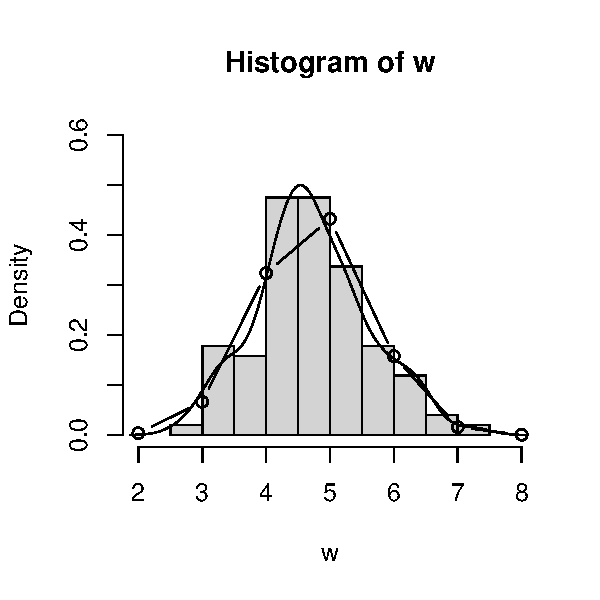
\includegraphics[scale=0.7]{1-4.pdf}
            \caption{题4图}
        \end{figure}
        \summary\\
        由线条显示的曲线是密度估计曲线,而点和线交错显示的曲线是相应正态分布的概率密度曲线。密度估计曲线与正态分布的概率密度曲线有一定差别,但不是很大,可近似认为样本符合正态分布。
        \item
        \code
\begin{lstlisting}
w <- scan("ex1_5-data.txt")
# 绘制茎叶图
stem(w)
# 绘制箱线图
boxplot(w)
# 计算五数总括
fivenum(w)
\end{lstlisting}
        \out
\begin{lstlisting}
> stem(w)

  The decimal point is at the |

  12 | 069
  14 | 477901112223336899
  16 | 0111233446677902233345555567789
  18 | 001223338891123355579
  20 | 0005689003588
  22 | 089
  24 | 346816
  26 | 
  28 | 
  30 | 0
\end{lstlisting}
        \begin{figure}[H]
            \centering
            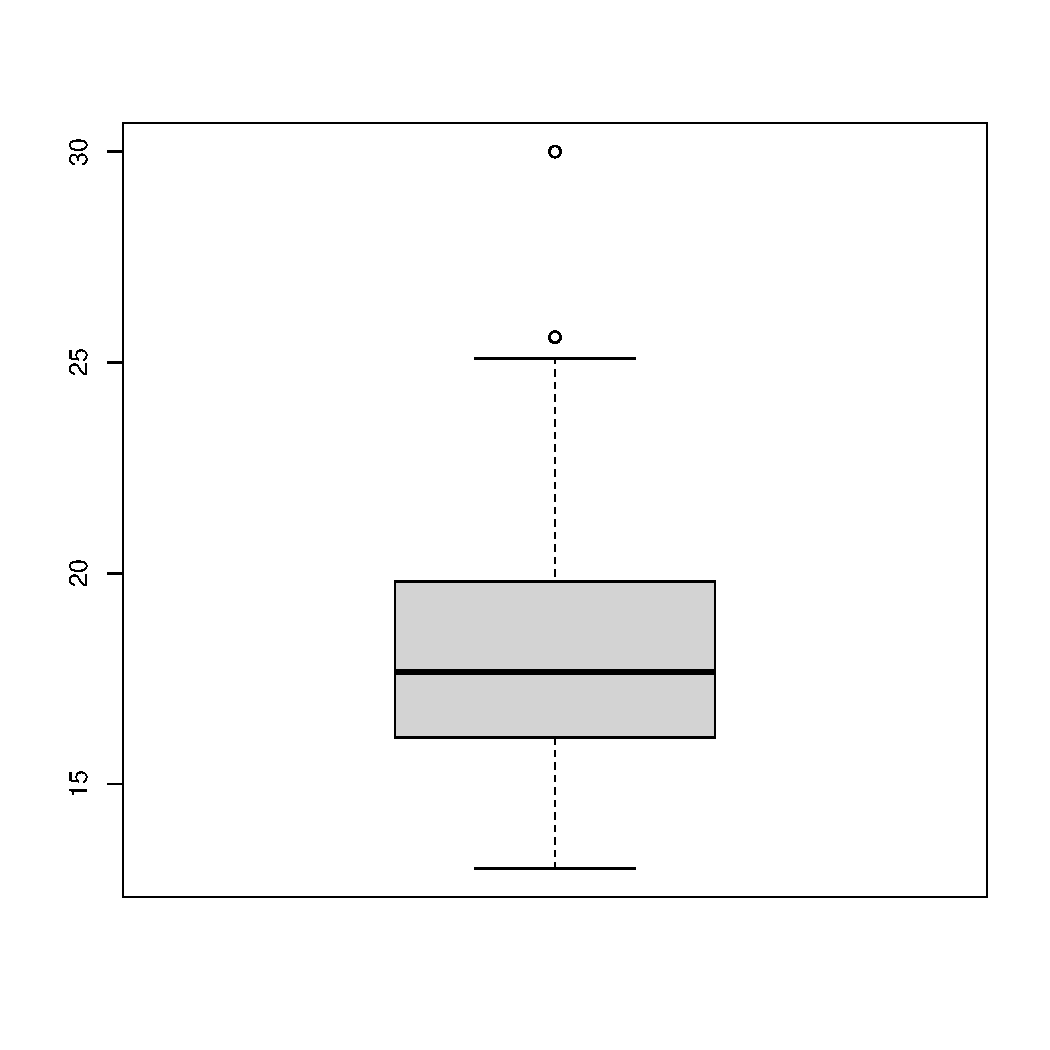
\includegraphics[scale=0.5]{1-5箱线图.pdf}
            \caption{题5箱线图}
        \end{figure}
\begin{lstlisting}
> fivenum(w)
[1] 13.00 16.10 17.65 19.80 30.00
\end{lstlisting}
        \summary
        \begin{enumerate}[label=(\arabic*)]
            \item 从茎叶图可以看出,绝大部分数据集中在$14 \sim 20$,在$16 \sim 18$形成一个高峰;数据分布不对称,有异常数据30.0;
            \item 从箱线图可以看出,数据存在异常值30.0,集中在较大值一侧,分布呈右偏态;
            \item 五数总括中,最小值为13.00,下四分位数为16.10,中位数为17.65,上四分位数为19.80,最大值为30.00。
        \end{enumerate}
        \item
        \code
\begin{lstlisting}
w <- scan("ex1_5-data.txt")
# 绘制经验分布函数曲线
plot(ecdf(w), verticals=TRUE, do.p=FALSE)
x <- 12:31
# 绘制正态分布函数曲线
lines(x, pnorm(x, mean(w), sd(w)))
\end{lstlisting}
        \out
        \begin{figure}[H]
            \centering
            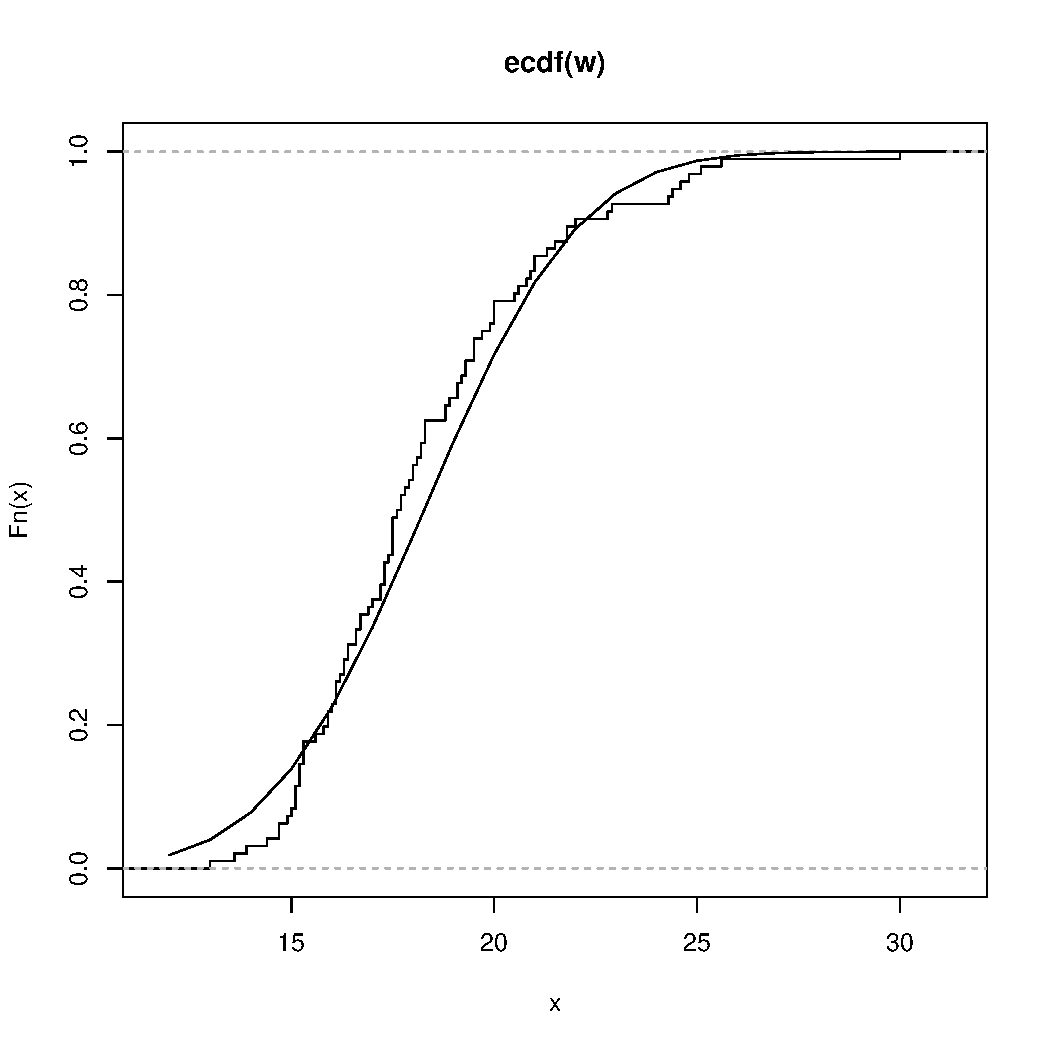
\includegraphics[scale=0.5]{1-6.pdf}
            \caption{题6图}
        \end{figure}
        \summary\\
        儿童体重的经验分布函数曲线用正态分布函数曲线拟合效果良好,可以认为数据来自正态总体。
        \item
        \code
\begin{lstlisting}
w <- scan("ex1_5-data.txt")
# 绘制正态QQ图
qqnorm(w)
qqline(w)
\end{lstlisting}
        \clearpage
        \out
        \begin{figure}[H]
            \centering
            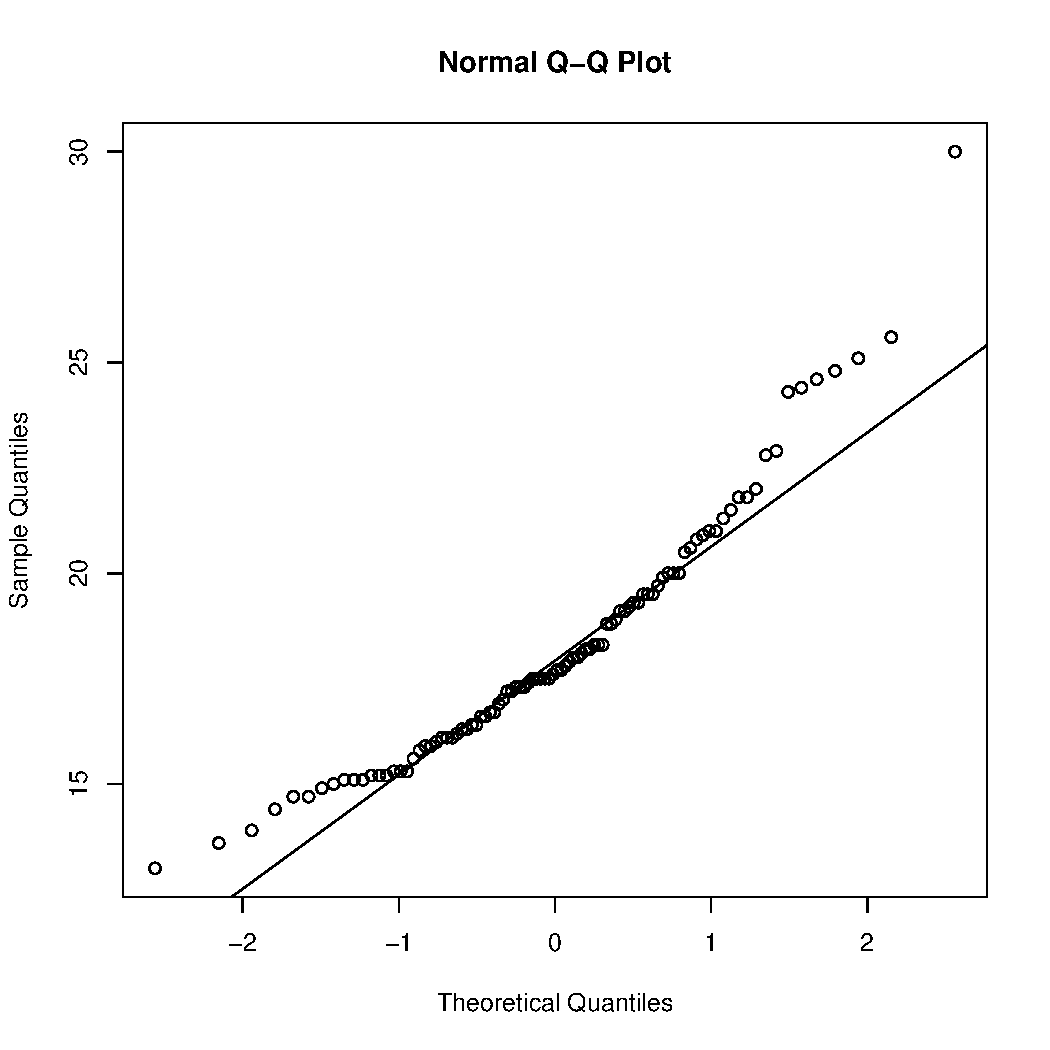
\includegraphics[scale=0.5]{1-7.pdf}
        \end{figure}
        \summary\\
        这些点中间部分近似在一条直线上,但首尾偏差较大,无法认为样本数据来自正态总体。
        \item
        \code
\begin{lstlisting}
w <- scan("ex1_5-data.txt")
n <- length(w);
k <- floor(1+3.3*log10(n));
R <- max(w) - min(w);
d <- round(R/k); d
A <- table(cut(w, br=c(13,15,17,19,21,23,30))); A
p <- pnorm(c(15,17,19,21,23,30), mean(w), sd(w));
p <- c(p[1],p[2]-p[1],p[3]-p[2],p[4]-p[3],p[5]-p[4],1-p[5]); p
chisq.test(A, p=p)
\end{lstlisting}
        \out
\begin{lstlisting}
> d <- round(R/k); d
[1] 2
> A <- table(cut(w, br=c(13,15,17,19,21,23,30))); A

(13,15] (15,17] (17,19] (19,21] (21,23] (23,30] 
      7      28      27      19       7       7 
> p <- c(p[1],p[2]-p[1],p[3]-p[2],p[4]-p[3],p[5]-p[4],1-p[5]); p
[1] 0.13841648 0.19775300 0.25927817 0.22211154 0.12430578 0.05813504
> chisq.test(A, p=p)

	Chi-squared test for given probabilities

data:  A
X-squared = 10.185, df = 5, p-value = 0.07016
\end{lstlisting}
        \summary\\
        $H_0:$来自正态总体,$H_1:$不来自正态总体,$p$值$= 0.07016 > 0.05$,则接受原假设,认为数据来自正态总体。
        \item
        \code
\begin{lstlisting}
red <- seq(420, 640, by = 20)
num <- c(2,4,7,16,20,20,24,22,16,2,6,1)
w <- rep(red, num)
ks.test(w, "pnorm", mean(w), sd(w))
\end{lstlisting}
        \out
\begin{lstlisting}
> ks.test(w, "pnorm", mean(w), sd(w))

	One-sample Kolmogorov-Smirnov test

data:  w
D = 0.10583, p-value = 0.0869
alternative hypothesis: two-sided

Warning message:
In ks.test(w, "pnorm", mean(w), sd(w)) :
  Kolmogorov - Smirnov检验里不应该有连结
\end{lstlisting}
        \summary\\
        $H_0:$数据来自正态总体,$H_1:$数据不是来自正态总体,$p$值为$0.0869>0.05$,则接受原假设,认为数据来自正态总体。
        \item
        \code
\begin{lstlisting}
w <- c(0.54,0.81,0.87,0.21,0.31,
       0.40,0.46,0.17,0.62,0.63,
       0.99,0.71,0.14,0.12,0.64,
       0.51,0.68,0.50,0.60,0.78)
# X^2拟合优度检验
A <- table(cut(w, br=c(0,0.2,0.4,0.6,0.8,1))); A
p <- punif(c(0.2,0.4,0.6,0.8,1), 0, 1);
p <- c(p[1],p[2]-p[1],p[3]-p[2],p[4]-p[3],1-p[4]); p
chisq.test(A, p=p)
# K-S检验
ks.test(w, "punif", 0, 1)
\end{lstlisting}
        \out
\begin{lstlisting}
> # X^2拟合优度检验
> A <- table(cut(w, br=c(0,0.2,0.4,0.6,0.8,1))); A

  (0,0.2] (0.2,0.4] (0.4,0.6] (0.6,0.8]   (0.8,1] 
        3         3         5         6         3 
> p <- c(p[1],p[2]-p[1],p[3]-p[2],p[4]-p[3],1-p[4]); p
[1] 0.2 0.2 0.2 0.2 0.2
> chisq.test(A, p=p)

	Chi-squared test for given probabilities

data:  A
X-squared = 2, df = 4, p-value = 0.7358

Warning message:
In chisq.test(A, p = p) : Chi-squared近似算法有可能不准
> # K-S检验
> ks.test(w, "punif", 0, 1)

	One-sample Kolmogorov-Smirnov test

data:  w
D = 0.16, p-value = 0.6285
alternative hypothesis: two-sided
\end{lstlisting}
        \summary
        \begin{enumerate}[label=(\arabic*)]
            \item $H_0:$来自$[0,1]$上的均匀分布,$H_1:$不来自$[0,1]$上的均匀分布,$\chi^2$拟合优度检验的$p$值为$0.7358>0.05$,则接受原假设,认为数据来自$[0,1]$上的均匀分布。
            \item $H_0:$来自$[0,1]$上的均匀分布,$H_1:$不来自$[0,1]$上的均匀分布,K-S检验的$p$值为$0.6285>0.05$,则接受原假设,认为数据来自$[0,1]$上的均匀分布。
        \end{enumerate}
        \item
        \code
\begin{lstlisting}
w <- c(36,32,16,15,35)
p <- c(0.2,0.2,0.2,0.2,0.2)
chisq.test(w, p=p)
\end{lstlisting}
        \out
\begin{lstlisting}
> chisq.test(w, p=p)

	Chi-squared test for given probabilities

data:  w
X-squared = 16.224, df = 4, p-value = 0.002733
\end{lstlisting}
        \summary\\
        $H_0:$不合格率相同,$H_1:$不合格率不相同,$p$值为$0.002733<0.05$,则拒绝原假设,认为五个工作日的产品不合格率不相同。
        \item
        \code
\begin{lstlisting}
w <- c(36,32,16,15,35)
p <- c(0.3,0.25,0.1,0.1,0.25)
chisq.test(w, p=p)
\end{lstlisting}
        \out
\begin{lstlisting}
> chisq.test(w, p=p)

	Chi-squared test for given probabilities

data:  w
X-squared = 1.2687, df = 4, p-value = 0.8667
\end{lstlisting}
        \summary\\
        $H_0:$这种说法正确,$H_1:$这种说法不正确,$p$值为$0.8667>0.05$,则接受原假设,认为这种说法正确。
    \end{enumerate}
\clearpage
    \section{非参数统计}
    \begin{enumerate}
        \item
        \code
\begin{lstlisting}
library(tseries)
w <- c(9.8,10.1,9.7,9.9,10,10,9.8,9.7,9.8,9.9)
binom.test(sum(w>10), sum(w<10)+sum(w>10), al='two.sided')
\end{lstlisting}
        \out
\begin{lstlisting}
> binom.test(sum(w>10), sum(w<10)+sum(w>10), al='two.sided')

	Exact binomial test

data:  sum(w > 10) and sum(w < 10) + sum(w > 10)
number of successes = 1, number of trials = 8, p-value = 0.07031
alternative hypothesis: true probability of success is not equal to 0.5
95 percent confidence interval:
 0.003159724 0.526509671
sample estimates:
probability of success 
                 0.125
\end{lstlisting}
        \summary\\
        $H_0:$中位数$=10$,不需要调整,$H_1:$中位数$\neq 10$,需要调整,$p$值为$0.07031>0.05$,则接受原假设,认为不需要调整。
        \item
        \code
\begin{lstlisting}
library(tseries)
w <- c(432.00,82.46,46.19,43.14,
       21.59,12.61,23.61,22.20,
       11.31,105.53,83.57,21.77,
       11.95,42.17,6.30,39.03)
binom.test(sum(w>32.32), sum(w<32.32)+sum(w>32.32), al='greater')
\end{lstlisting}
        \out
\begin{lstlisting}
> binom.test(sum(w>32.32), sum(w<32.32)+sum(w>32.32), al='greater')

	Exact binomial test

data:  sum(w > 32.32) and sum(w < 32.32) + sum(w > 32.32)
number of successes = 8, number of trials = 16, p-value = 0.5982
alternative hypothesis: true probability of success is greater than 0.5
95 percent confidence interval:
 0.2786027 1.0000000
sample estimates:
probability of success 
                   0.5 
\end{lstlisting}
        \summary\\
        $H_0:$中位数并无增加,$H_1:$中位数有所增加,$p$值为$0.5982>0.05$,则接受原假设,认为中位数并无增加。
        \item
        \code
\begin{lstlisting}
library(tseries)
x <- c(2.300,2.396,2.100,2.442,1.81,2.007,1.766,1.224,1.411,1.438,0.892,1.167)
D <- numeric()
if(length(x)%%2==0){
	c=length(x)/2
	for(i in 1:c)
		D[i]=x[i]-x[i+c]}
if(length(x)%%2==1){
	c=(length(x)+1)/2
	for(i in 1:c-1)
		D[i]=x[i]-x[i+c]}
binom.test(sum(D>0), sum(D<0)+sum(D>0), al='less')
\end{lstlisting}
        \out
\begin{lstlisting}
> binom.test(sum(D>0), sum(D<0)+sum(D>0), al='less')

	Exact binomial test

data:  sum(D > 0) and sum(D < 0) + sum(D > 0)
number of successes = 6, number of trials = 6, p-value = 1
alternative hypothesis: true probability of success is less than 0.5
95 percent confidence interval:
 0 1
sample estimates:
probability of success 
                     1 
\end{lstlisting}
        \summary\\
        $H_0:M \geq 0$,无上升趋势,$H_1:M < 0$,有上升趋势,$p$值为$1>0.05$,则接受原假设,认为销售量没有单调增加趋势。
        \item
        \code
\begin{lstlisting}
library(tseries)
w <- c(3.6,3.9,4.1,3.6,3.8,3.7,3.4,4.0,3.8,4.1,3.9,4.0,3.8,4.2,4.1)
x <- numeric()
for(i in 1:length(w)){
    if(w[i]-median(w)>0)
	x[i]=1
	if(w[i]-median(w)<=0)
	x[i]=0}
x <- factor(x)
runs.test(x)
\end{lstlisting}
        \out
\begin{lstlisting}
> runs.test(x)

	Runs Test

data:  x
Standard Normal = 1.008, p-value = 0.3134
alternative hypothesis: two.sided
\end{lstlisting}
        \summary\\
        $H_0:$质量的变动是随机的,$H_1:$质量的变动不是随机的,$p$值为$0.3134>0.05$,则接受原假设,认为质量的变动是随机的。
        \item
        \code
\begin{lstlisting}
library(tseries)
w <- c(11,19,17,15,15,16,193)
x <- numeric()
for(i in 1:length(w)){
    if(w[i]-median(w)>0)
	x[i]=1
	if(w[i]-median(w)<=0)
	x[i]=0}
x <- factor(x)
runs.test(x)
\end{lstlisting}
        \out
\begin{lstlisting}
> runs.test(x)

	Runs Test

data:  x
Standard Normal = -0.3638, p-value = 0.716
alternative hypothesis: two.sided
\end{lstlisting}
        \summary\\
        $H_0:$一周内各日的死亡数是随机的,$H_1:$一周内各日的死亡数不是随机的,$p$值为$0.716>0.05$,则接受原假设,认为一周内各日的死亡数是随机的。
        \item
        \code
\begin{lstlisting}
x <- c(54.0,55.1,53.8,54.2,52.1,54.2,55.0,55.8,55.1,55.3)
wilcox.test(x, alternative="two.sided", mu=54, exact=FALSE, conf.level=0.95)
\end{lstlisting}
        \out
\begin{lstlisting}
> wilcox.test(x, alternative="two.sided", mu=54, exact=FALSE, conf.level=0.95)

	Wilcoxon signed rank test with continuity correction

data:  x
V = 34, p-value = 0.1906
alternative hypothesis: true location is not equal to 54
\end{lstlisting}
        \summary\\
        $H_0:$零件质量正常,等于54克,$H_1:$零件质量不正常,不等于54克,$p$值为$0.1906>0.05$,则接受原假设,认为零件质量正常。
        \item
        \code
\begin{lstlisting}
dcxfp <- c(0.6,1.2,2.0,2.4,3.1,4.1,5.0,5.9,7.4,13.9)
pzczdz <- c(9.8,10.2,10.6,13.0,14.0,14.8,15.6,15.6,21.6,24.0)
wilcox.test(pzczdz, dcxfp, alternative="l", paired=FALSE, exact=FALSE)
\end{lstlisting}
        \out
\begin{lstlisting}
> wilcox.test(pzczdz, dcxfp, alternative="l", paired=FALSE, exact=FALSE)

	Wilcoxon rank sum test with continuity correction

data:  pzczdz and dcxfp
W = 96, p-value = 0.9998
alternative hypothesis: true location shift is less than 0
\end{lstlisting}
        \summary\\
        $H_0:$皮质醇增多症的血浆总皮醇测定值高于单纯性肥胖,$H_1:$皮质醇增多症的血浆总皮醇测定值不高于单纯性肥胖,$p$值为$0.9998>0.05$,则接受原假设,认为皮质醇增多症的血浆总皮醇测定值高于单纯性肥胖。
        \item
        \code
\begin{lstlisting}
zf <- c(8.2,10.7,7.5,14.6,6.3,9.2,11.9,5.6,12.8,5.2,4.9,13.5)
jk <- c(4.7,6.3,5.2,6.8,5.6,4.2,6.0,7.4,8.1,6.5)
ansari.test(zf, jk, alternative="two.sided", exact=F, conf.level=0.95)
\end{lstlisting}
        \out
\begin{lstlisting}
> ansari.test(zf, jk, alternative="two.sided", exact=F, conf.level=0.95)

	Ansari-Bradley test

data:  zf and jk
AB = 60.5, p-value = 0.1269
alternative hypothesis: true ratio of scales is not equal to 1
\end{lstlisting}
        \summary\\
        $H_0:$尿酸浓度的变异相同,$H_1:$尿酸浓度的变异不同,$p$值为$0.1269>0.05$,则接受原假设,认为尿酸浓度的变异相同。
        \item
        \code
\begin{lstlisting}
x <- c(55,74,68,80,77,69,57,72,63,52,85,66,71,48,83,78,51,67)
y <- c(41,64,61,70,75,60,53,59,61,48,79,65,70,47,81,69,50,62)
d <- x-y
# 符号检验
binom.test(sum(d>5), sum(d>5)+sum(d<5), al="two.sided")
# Wilcoxon符号秩检验
wilcox.test(x-5, y, alternative="two.sided", paired=T, exact=F, correct=F)
\end{lstlisting}
        \out
\begin{lstlisting}
> # 符号检验
> binom.test(sum(d>5), sum(d>5)+sum(d<5), al="two.sided")

	Exact binomial test

data:  sum(d > 5) and sum(d > 5) + sum(d < 5)
number of successes = 8, number of trials = 17, p-value = 1
alternative hypothesis: true probability of success is not equal to 0.5
95 percent confidence interval:
 0.2298327 0.7218817
sample estimates:
probability of success 
             0.4705882 

> # Wilcoxon符号秩检验
> wilcox.test(x-5, y, alternative="two.sided", paired=T, exact=F, correct=F)

	Wilcoxon signed rank test

data:  x - 5 and y
V = 89, p-value = 0.5516
alternative hypothesis: true location shift is not equal to 0
\end{lstlisting}
        \summary\\
        $H_0:$城市噪音已下降5分贝,$H_1:$城市噪音没有下降5分贝,
        \begin{enumerate}[label=(\arabic*)]
          \item 符号检验的$p$值为$1>0.05$,则接受原假设,认为城市噪音已下降5分贝。
          \item Wilcoxon符号秩检验的$p$值为$0.5516>0.05$,则接受原假设,认为城市噪音已下降5分贝。
        \end{enumerate}
        综上,接受原假设,认为城市噪音已下降5分贝。
        \item
        \code
\begin{lstlisting}
pjz <- c(83.46,49.25,70.21,50.06,43.83,44.03,
         43.59,43.61,42.57,55.71,52.85,
         44.61,45.28,46.37,42.19,42.43)
jj <- c(5118,3148,2574,2216,2186,1759,
        1829,2008,1514,3939,2865,3156,
        1816,2530,2476,2651)
cor.test(pjz, jj, alternative="two.sided", method="spearman")
\end{lstlisting}
        \out
\begin{lstlisting}
> cor.test(pjz, jj, alternative="two.sided", method="spearman")

	Spearman's rank correlation rho

data:  pjz and jj
S = 288, p-value = 0.02156
alternative hypothesis: true rho is not equal to 0
sample estimates:
      rho 
0.5764706 
\end{lstlisting}
        \summary\\
        $H_0:$二者不相关,$H_1:$二者相关,$p$值为$0.02156<0.05$,则拒绝原假设,认为二者相关,相关系数为0.5764706。
        \item
        \code
\begin{lstlisting}
pjz <- c(83.46,49.25,70.21,50.06,43.83,44.03,
         43.59,43.61,42.57,55.71,52.85,
         44.61,45.28,46.37,42.19,42.43)
jj <- c(5118,3148,2574,2216,2186,1759,
        1829,2008,1514,3939,2865,3156,
        1816,2530,2476,2651)
cor.test(pjz, jj, alternative="two.sided", method="kendall", exact=F)
\end{lstlisting}
        \out
\begin{lstlisting}
> cor.test(pjz, jj, alternative="two.sided", method="kendall", exact=F)

	Kendall's rank correlation tau

data:  pjz and jj
z = 2.3412, p-value = 0.01922
alternative hypothesis: true tau is not equal to 0
sample estimates:
      tau 
0.4333333 
\end{lstlisting}
        \summary\\
        $H_0:$二者不相关,$H_1:$二者相关,$p$值为$0.01922<0.05$,则拒绝原假设,认为二者相关,相关系数为0.4333333。
        \item
        \code
\begin{lstlisting}
x <- matrix(c(15,13,20,18), nr=2)
chisq.test(x, correct=F)
\end{lstlisting}
        \out
\begin{lstlisting}
> chisq.test(x, correct=F)

	Pearson's Chi-squared test

data:  x
X-squared = 0.0057171, df = 1, p-value = 0.9397
\end{lstlisting}
        \summary\\
        $H_0:$体育达标水平与性别相互独立,即无关,$H_1:$体育达标水平与性别不独立,即有关,$p$值为$0.9397>0.05$,则接受原假设,认为体育达标水平与性别相互独立,即无关。
    \end{enumerate}
\clearpage
    \section{多元统计分析相关基础}
    \begin{enumerate}
        \item
        \code
\begin{lstlisting}
library(ICSNP)
boy <- read.table("data.exam3.4.1.txt", header=TRUE)
mu0 <- c(155,38,2205)
# 取F统计量
HotellingsT2(boy, mu=mu0, test="f")
# 取X^2统计量
HotellingsT2(boy, mu=mu0, test="chi")
\end{lstlisting}
        \out
\begin{lstlisting}
> # 取F统计量
> HotellingsT2(boy, mu=mu0, test="f")

	Hotelling's one sample T2-test

data:  boy
T.2 = 1.3725, df1 = 3, df2 = 26, p-value = 0.2732
alternative hypothesis: true location is not equal to c(155,38,2205)

> # 取X^2统计量
> HotellingsT2(boy, mu=mu0, test="chi")

	Hotelling's one sample T2-test

data:  boy
T.2 = 4.4343, df = 3, p-value = 0.2182
alternative hypothesis: true location is not equal to c(155,38,2205)
\end{lstlisting}
        \summary\\
        $H_0:$数据均值向量等于$(155,38,2205)^{\mathrm{T}}$,$H_1:$数据均值向量不等于$(155,38,2205)^{\mathrm{T}}$,
        \begin{enumerate}[label=(\arabic*)]
            \item 用统计量$F$检验,$p$值为$0.2732>0.05$,则接受原假设,认为数据均值向量等于$(155,38,2205)^{\mathrm{T}}$。
            \item 用统计量$\chi^2$检验,$p$值为$0.2182>0.05$,则接受原假设,认为数据均值向量等于$(155,38,2205)^{\mathrm{T}}$。
        \end{enumerate}
        综上,接受原假设,认为数据均值向量等于$(155,38,2205)^{\mathrm{T}}$。
        \item
        \code
\begin{lstlisting}
A <- matrix(c(0.702,0.541,0.184,0.253,
              0.541,0.712,0.228,0.258,
              0.184,0.228,0.392,0.346,
              0.253,0.258,0.346,0.806), nr=4)
mu0 <- c(22.75,32.75,51.50,61.50)
x0 <- c(22.82,32.79,51.45,61.38)
n <- 21
p <- 4
T2 <- (n-1)*n*t(x0-mu0)%*%solve(A)%*%(x0-mu0);
F <- (n-p)/((n-1)*p)*T2;
pvf <- 1 - pf(F,p,n-p); pvf
\end{lstlisting}
        \out
\begin{lstlisting}
> pvf <- 1 - pf(F,p,n-p); pvf
           [,1]
[1,] 0.03538181
\end{lstlisting}
        \summary\\
        $H_0:\pmb{\mu}=\pmb{\mu}_0,H_1:\pmb{\mu} \neq \pmb{\mu}_0$,$p$值为$0.03538181<0.05$,则拒绝原假设,认为$\pmb{\mu} \neq \pmb{\mu}_0$。
        \item
        \code
\begin{lstlisting}
library(ICSNP)
# (1)
s_ve <- as.matrix(iris[1:100,1:4]);
s_ve_G <- as.factor(iris[1:100,5]);
HotellingsT2(s_ve~s_ve_G)
# (2)
ve_vi <- as.matrix(iris[51:150,1:4]);
ve_vi_G <- as.factor(iris[51:150,5]);
HotellingsT2(ve_vi~ve_vi_G)
# (3)
# setosa
setosa <- as.matrix(iris[1:50,1:4]);
# versicolor
versicolor <- as.matrix(iris[51:100,1:4]);
# vinginica
vinginica <- as.matrix(iris[101:150,1:4]);
n <- 50
p <- 4
avg_s <- as.matrix(colSums(setosa)/50);
avg_ve <- as.matrix(colSums(versicolor)/50);
avg_vi <- as.matrix(colSums(vinginica)/50);
avg <- (avg_s + avg_ve + avg_vi)/3;
A <- 50*(avg_s - avg) %*% t(avg_s - avg) + 50*(avg_ve - avg) %*% t(avg_ve - avg) + 50*(avg_vi - avg) %*% t(avg_vi - avg);
E <- matrix(0,4,4);
for (i in seq(1,n)){
	E = E + (t(t(setosa[i,])) - avg_s) %*% t(t(t(setosa[i,])) - avg_s);
}
for (i in seq(1,n)){
	E = E + (t(t(versicolor[i,])) - avg_ve) %*% t(t(t(versicolor[i,])) - avg_ve);
}
for (i in seq(1,n)){
	E = E + (t(t(vinginica[i,])) - avg_vi) %*% t(t(t(vinginica[i,])) - avg_vi);
}
Lambda <- det(E)/(det(E+A));
pvf3 <- 1-pf((150-3-4+1)/4 * (1 - sqrt(Lambda))/sqrt(Lambda), 8, 2*(150-3-4+1)); pvf3
\end{lstlisting}
        \out
\begin{lstlisting}
> # (1)
> HotellingsT2(s_ve~s_ve_G)

	Hotelling's two sample T2-test

data:  s_ve by s_ve_G
T.2 = 625.46, df1 = 4, df2 = 95, p-value < 2.2e-16
alternative hypothesis: true location difference is not equal to c(0,0,0,0)

> # (2)
> HotellingsT2(ve_vi~ve_vi_G)

	Hotelling's two sample T2-test

data:  ve_vi by ve_vi_G
T.2 = 86.148, df1 = 4, df2 = 95, p-value < 2.2e-16
alternative hypothesis: true location difference is not equal to c(0,0,0,0)

> # (3)
> pvf3
[1] 0
\end{lstlisting}
        \summary
        \begin{enumerate}[label=(\arabic*)]
            \item $H_0:\mu_{setosa}=\mu_{versicolor},H_1:\mu_{setosa} \neq \mu_{versicolor}$,$p$值$< 2.2\times 10^{-16}<0.05$,则拒绝原假设,认为setosa与versicolor的均值向量不相等。
            \item $H_0:\mu_{versicolor}=\mu_{vinginica},H_1:\mu_{versicolor} \neq \mu_{vinginica}$,$p$值$< 2.2\times 10^{-16}<0.05$,则拒绝原假设,认为versicolor与vinginica的均值向量不相等。
            \item $H_0:$三种花的均值向量相等,$H_1:$三种花的均值向量不相等,$p$值为$0<0.05$,则拒绝原假设,认为三种花的均值向量不相等。
        \end{enumerate}
        \item
        \code
\begin{lstlisting}
x <- read.table("ex3_4-data.txt", header=TRUE, row.names=1)
# 均值向量
colMeans(x)
# 协方差矩阵
cov(x)
# 相关系数矩阵
cor(x)
\end{lstlisting}
        \out
\begin{lstlisting}
> # 均值向量
> colMeans(x)
         X1          X2          X3          X4          X5          X6 
 1487.42125   685.85438 10874.18750   449.13000    58.87375    62.83937 
> # 协方差矩阵
> cov(x)
           X1         X2        X3        X4          X5         X6
X1  2093336.6  841893.88  18479476  703207.2  118473.934  139988.10
X2   841893.9  350404.23   7036375  277089.8   48305.919   54154.89
X3 18479475.7 7036374.81 212249748 6910248.0 1017813.524 1424766.40
X4   703207.2  277089.84   6910248  250159.3   38767.802   50785.80
X5   118473.9   48305.92   1017814   38767.8    7008.546    7660.30
X6   139988.1   54154.89   1424766   50785.8    7660.300   10541.30
> # 相关系数矩阵
> cor(x)
          X1        X2        X3        X4        X5        X6
X1 1.0000000 0.9829992 0.8766909 0.9717521 0.9781137 0.9423764
X2 0.9829992 1.0000000 0.8159071 0.9358961 0.9747690 0.8910577
X3 0.8766909 0.8159071 1.0000000 0.9483349 0.8345083 0.9525174
X4 0.9717521 0.9358961 0.9483349 1.0000000 0.9258677 0.9889784
X5 0.9781137 0.9747690 0.8345083 0.9258677 1.0000000 0.8912195
X6 0.9423764 0.8910577 0.9525174 0.9889784 0.8912195 1.0000000
\end{lstlisting}
        \summary
        \begin{enumerate}[label=(\arabic*)]
            \item 数据的均值向量为
            \[(1487.42125,685.85438,10874.18750,449.13000,58.87375,62.83937)^{\mathrm{T}}\]
            \item 数据的协方差矩阵为
            \[\begin{pmatrix}
                2093336.6 & 841893.88 & 18479476 & 703207.2 & 118473.934 & 139988.10 \\
                841893.9 & 350404.23  & 7036375 & 277089.8 &  48305.919  & 54154.89 \\
                18479475.7 & 7036374.81 & 212249748 & 6910248.0 & 1017813.524 & 1424766.40 \\
                703207.2 & 277089.84 &  6910248 & 250159.3  & 38767.802  & 50785.80 \\
                118473.9 &  48305.92 &  1017814  & 38767.8  &  7008.546  &  7660.30 \\
                139988.1 &  54154.89  & 1424766 &  50785.8  &  7660.300 &  10541.30
            \end{pmatrix}\]
            \item 数据的相关系数矩阵为
            \[\begin{pmatrix}
                1.0000000 & 0.9829992 & 0.8766909 & 0.9717521 & 0.9781137 & 0.9423764 \\
                0.9829992 & 1.0000000 & 0.8159071 & 0.9358961 & 0.9747690 & 0.8910577 \\
                0.8766909 & 0.8159071 & 1.0000000 & 0.9483349 & 0.8345083 & 0.9525174 \\
                0.9717521 & 0.9358961 & 0.9483349 & 1.0000000 & 0.9258677 & 0.9889784 \\
                0.9781137 & 0.9747690 & 0.8345083 & 0.9258677 & 1.0000000 & 0.8912195 \\
                0.9423764 & 0.8910577 & 0.9525174 & 0.9889784 & 0.8912195 & 1.0000000
            \end{pmatrix}\]
        \end{enumerate}
        \item
        \code
\begin{lstlisting}
data <- read.table("ex3_4-data.txt", header=TRUE, row.names=1)
x <- data[2:5,]
# 轮廓图
source("outline.R")
outline(x)
# 蛛网图
source("spider.R")
spider(x)
# 调和曲线图
source("harmonic.curve.R")
harmonic.curve(x)
\end{lstlisting}
        \clearpage
        \out
        \begin{figure}[H]
            \centering
            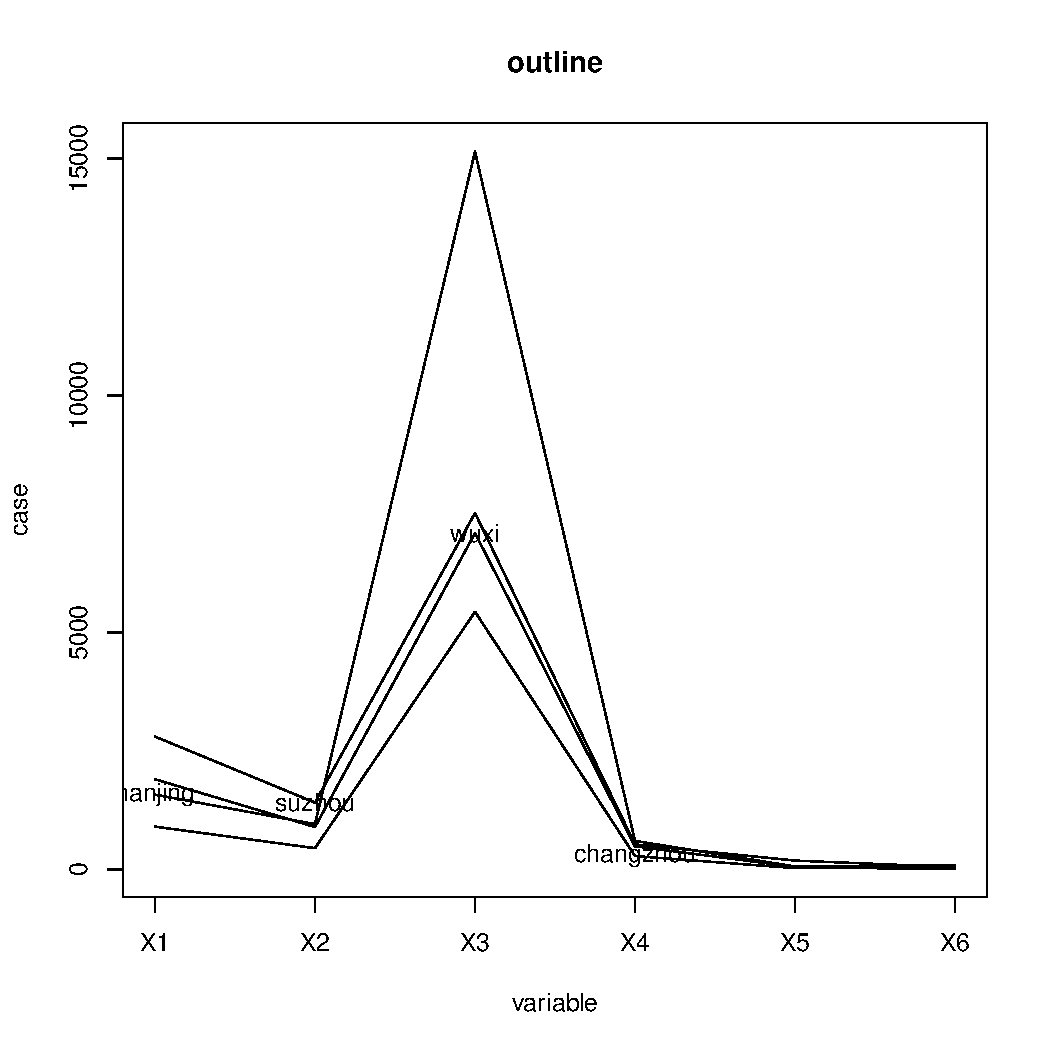
\includegraphics[scale=0.4]{3-5轮廓图.pdf}
            \caption{题5轮廓图}
        \end{figure}
        \begin{figure}[H]
          \centering
            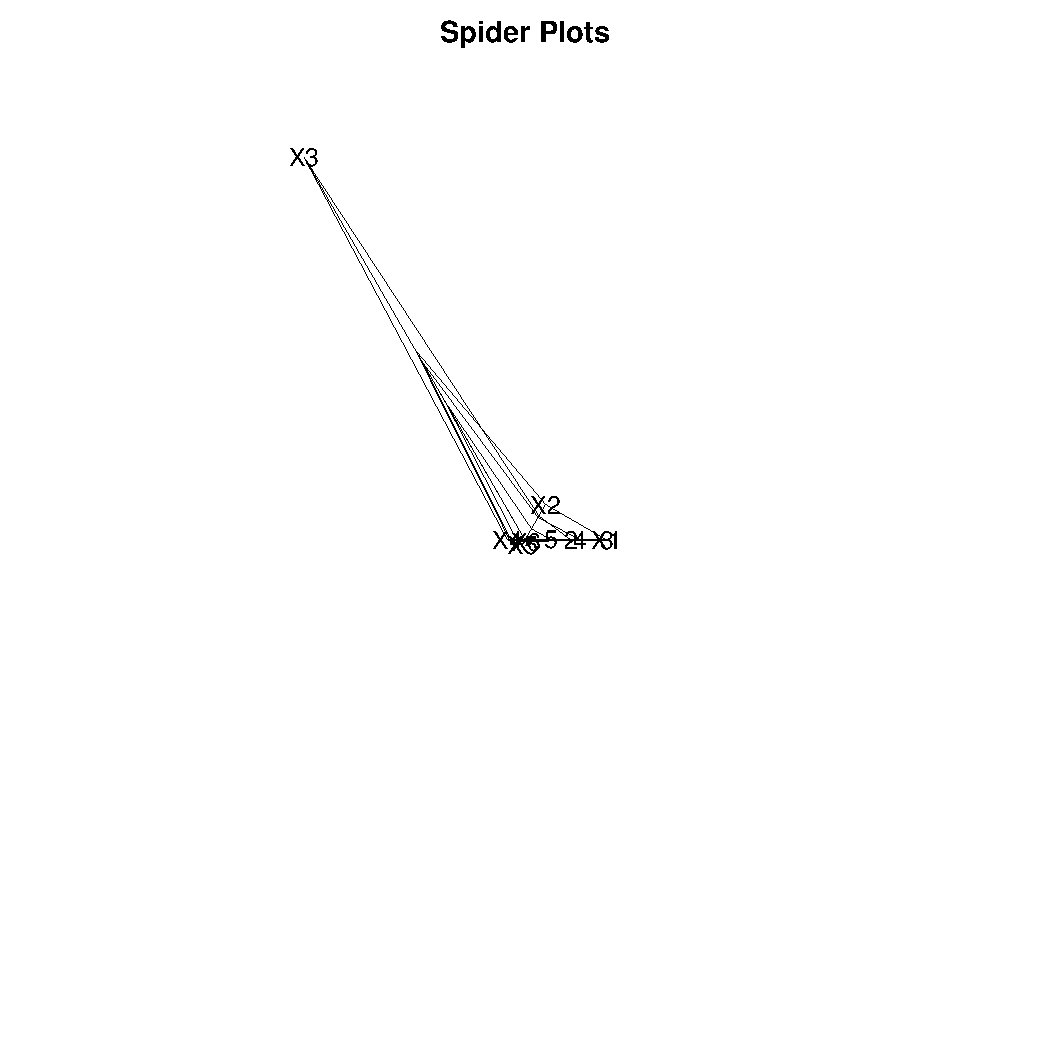
\includegraphics[scale=0.4]{3-5蛛网图.pdf}
            \caption{题5蛛网图}
        \end{figure}
        \begin{figure}[H]
          \centering
            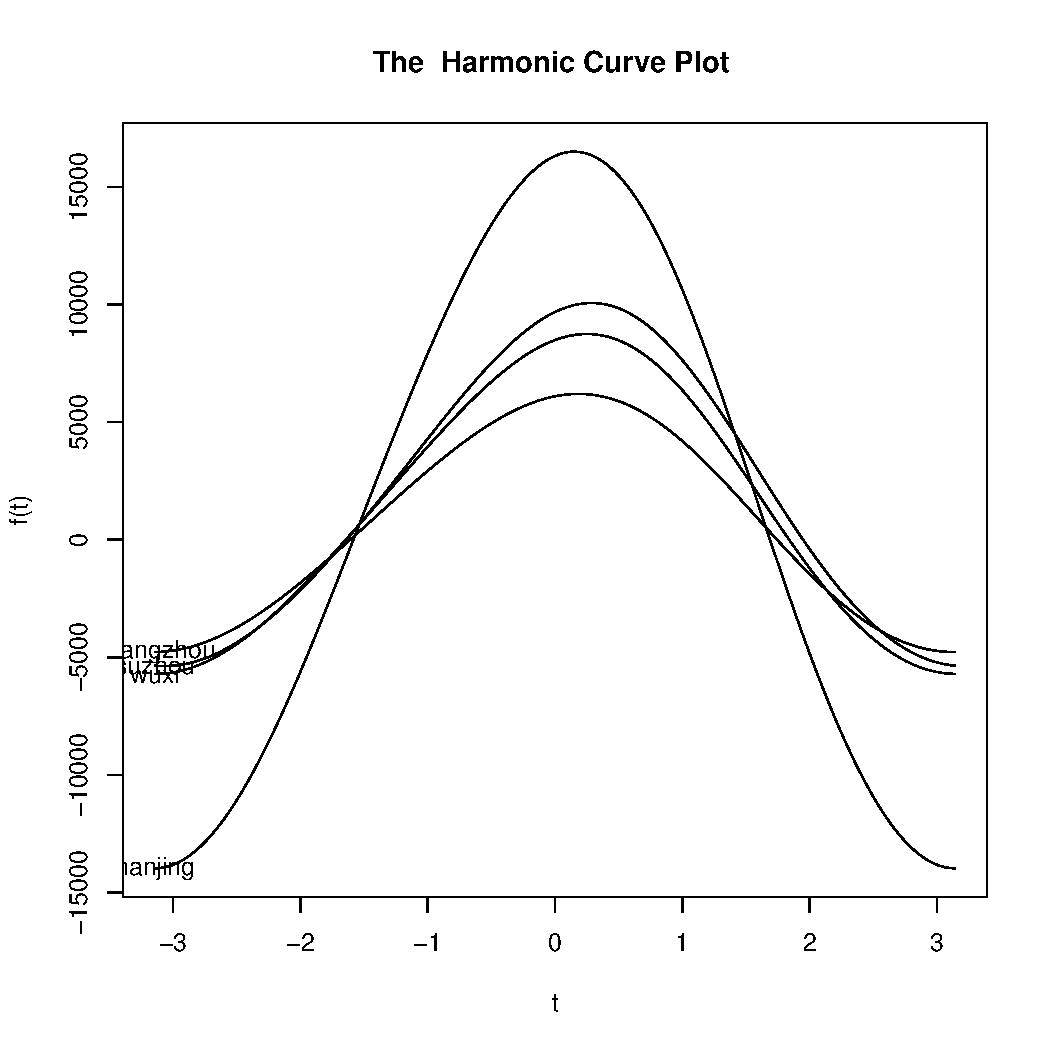
\includegraphics[scale=0.4]{3-5调和曲线图.pdf}
            \caption{题5调和曲线图}
        \end{figure}
    \end{enumerate}
\clearpage
    \section{回归分析}
    \begin{enumerate}
        \item
        \code
\begin{lstlisting}
x <- read.table("ex4_1-data.txt", header=TRUE)
lm.1 <- lm(Y~X1+X2, data=x)
summary(lm.1)
R = sqrt(summary(lm(Y~X1+X2, data=x))$r.sq); R
\end{lstlisting}
        \out
\begin{lstlisting}
> summary(lm.1)

Call:
lm(formula = Y ~ X1 + X2, data = x)

Residuals:
    Min      1Q  Median      3Q     Max 
-3.9340 -0.8672  0.5711  0.7114  4.4507 

Coefficients:
             Estimate Std. Error t value Pr(>|t|)    
(Intercept) -61.47289   17.60192  -3.492  0.00580 ** 
X1            2.12039    0.18148  11.684 3.75e-07 ***
X2            0.39431    0.08631   4.569  0.00103 ** 
---
Signif. codes:  0 ‘***’ 0.001 ‘**’ 0.01 ‘*’ 0.05 ‘.’ 0.1 ‘ ’ 1

Residual standard error: 2.968 on 10 degrees of freedom
Multiple R-squared:  0.9417,	Adjusted R-squared:  0.9301 
F-statistic: 80.83 on 2 and 10 DF,  p-value: 6.709e-07

> R
[1] 0.9704358
\end{lstlisting}
        \summary\\
        根据输出,可以得到
        \begin{enumerate}[label=(\arabic*)]
            \item $Y$关于$X_1,X_2$的二元线性回归方程为
            \[Y=-61.47289+2.12039X_1+0.39431X_2.\]
            \item 自变量$X_1$的系数$p$值为$3.75\times 10^{-7}<0.05$,认为$X_1$在0.05的显著性水平下是显著的;\\自变量$X_2$的系数$p$值为$0.00103<0.05$,认为$X_2$在0.05的显著性水平下是显著的;
            \item 复相关系数为0.9704358。
        \end{enumerate}
        \item
        \code
\begin{lstlisting}
x <- read.table("ex4_2-data.txt", header=TRUE)
# (1)
lm.1 <- lm(Y~X1+X2, data=x)
coefficients(lm.1)
# (2)
attach(x)
# 散点图
plot(Y~X1)
abline(lm(Y~X1))
plot(Y~X2)
abline(lm(Y~X2))
# 残差图
resid <- residuals(lm.1)
y.pre <- predict(lm.1)
plot(y.pre, resid)
# 残差QQ图
plot(lm.1,2)
\end{lstlisting}
        \out
\begin{lstlisting}
> coefficients(lm.1)
(Intercept)          X1          X2 
 -4.9513762   1.5465083  -0.9539819
\end{lstlisting}
        \begin{figure}[H]
            \centering
            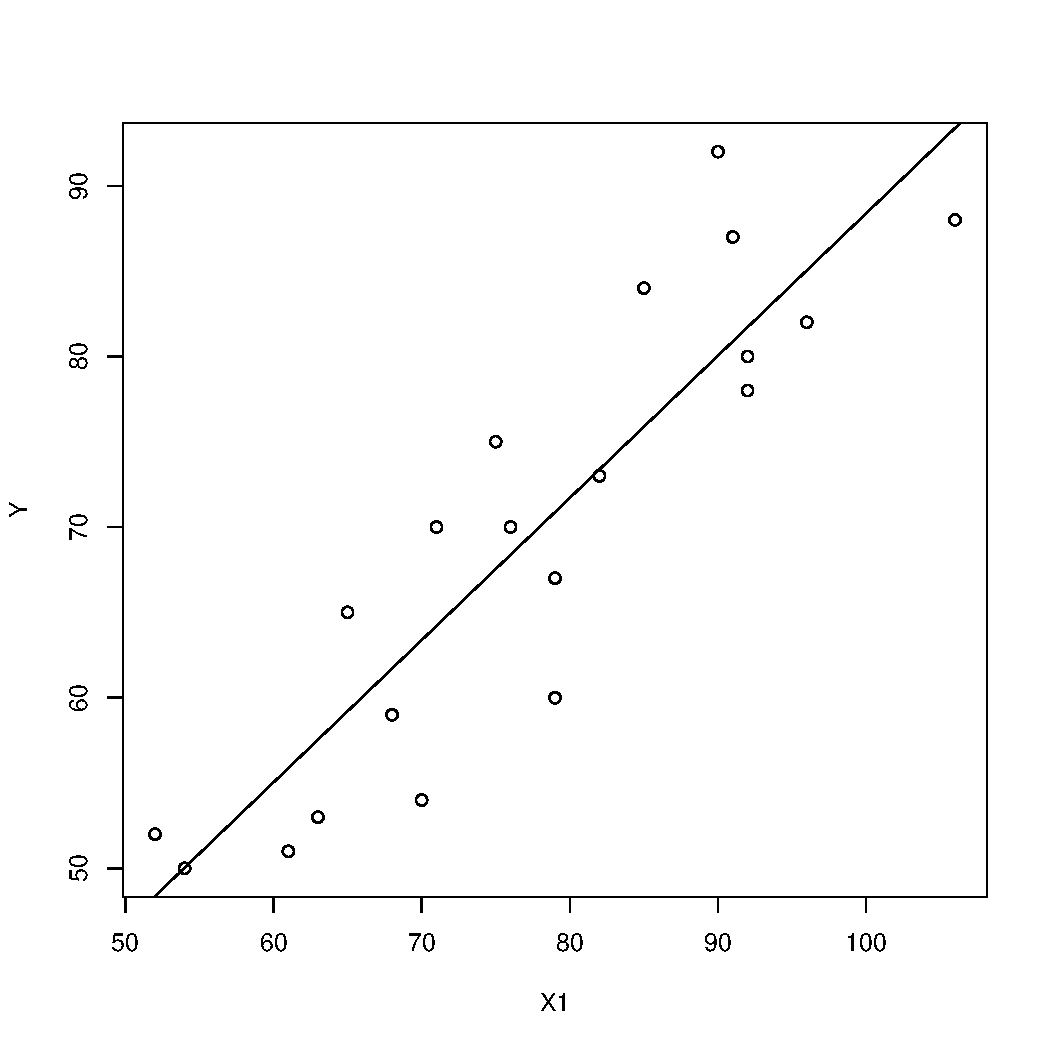
\includegraphics[scale=0.6]{4.2散点图Y-X1.pdf}
            \caption{题2中$Y$关于$X_1$的散点图}
        \end{figure}
        \begin{figure}[H]
            \centering
            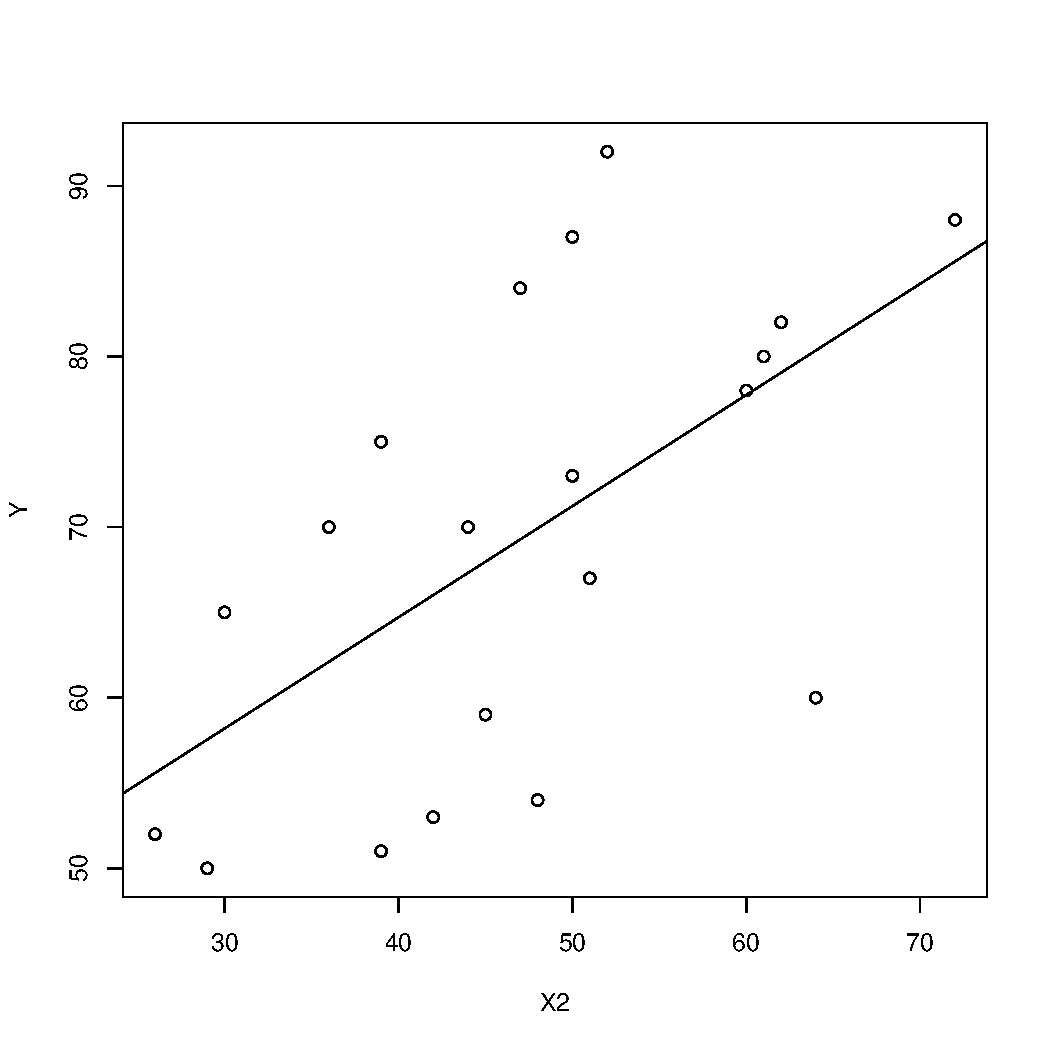
\includegraphics[scale=0.6]{4.2散点图Y-X2.pdf}
            \caption{题2中$Y$关于$X_2$的散点图}
        \end{figure}
        \begin{figure}[H]
            \centering
            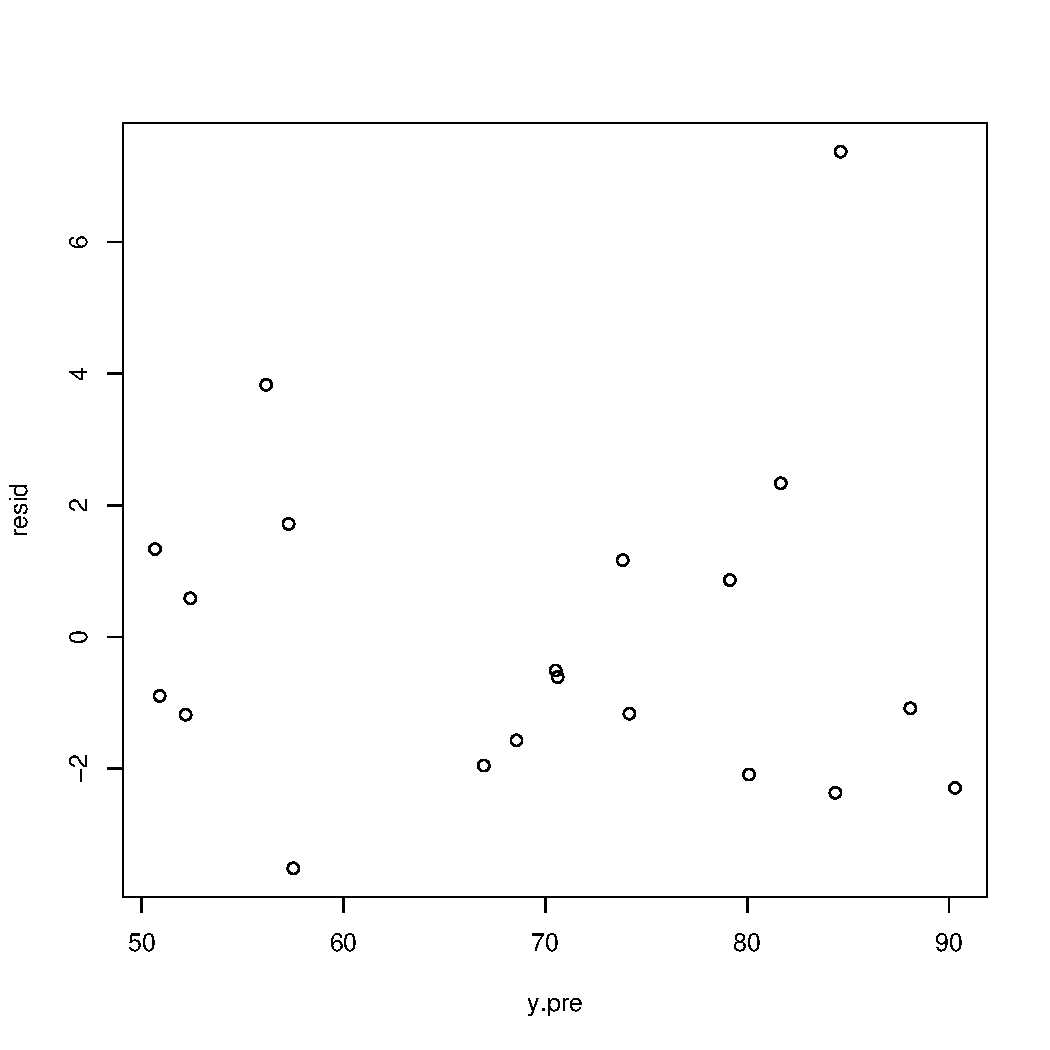
\includegraphics[scale=0.6]{4.2残差图.pdf}
            \caption{题2中的残差图}
        \end{figure}
        \begin{figure}[H]
            \centering
            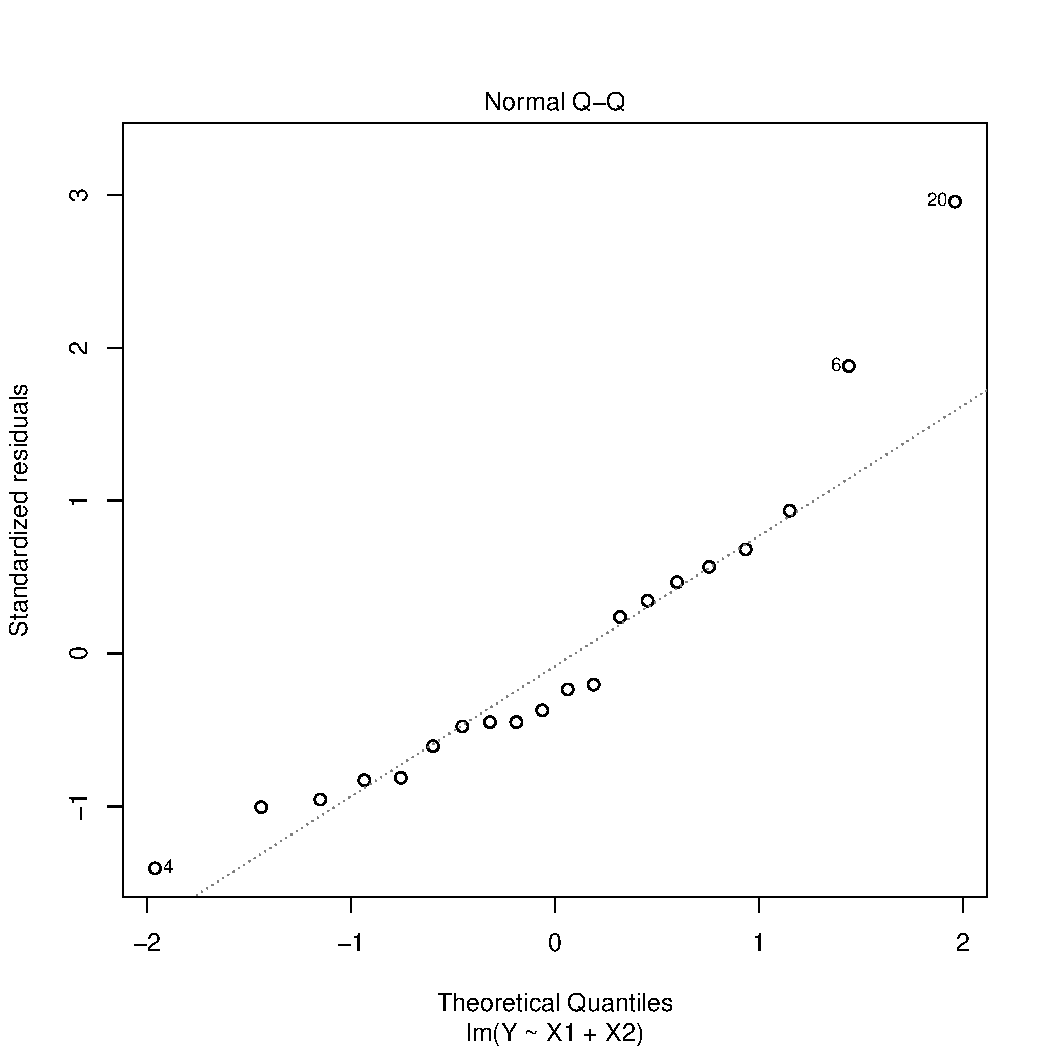
\includegraphics[scale=0.6]{4.2残差QQ图.pdf}
            \caption{题2中的残差QQ图}
        \end{figure}
        \summary\\
        根据输出,可以得到
        \begin{enumerate}[label=(\arabic*)]
            \item $Y$关于$X_1,X_2$的二元线性回归方程为
            \[Y=-4.9513762+1.5465083X_1-0.9539819X_2.\]
            \item 通过两张散点图和残差图,可以认为残差随时间变换呈线性变化,因此回归函数中应包含时间的线性项;\\
            通过残差QQ图,可以认为残差所属总体为$N(0,1)$,因此总体分布是正态分布。
        \end{enumerate}
        \item
        \code
\begin{lstlisting}
x <- read.table("ex4_3-data.txt", header=TRUE)
source("step.regression.R")
step.regression(x, x[[6]], c(2,3,4,5), 0.05, 0.05)
attach(x)
lm.1 <- lm(Y2~Y1+X3+X2, data=x)
summary(lm.1)
\end{lstlisting}
        \out
\begin{lstlisting}
> step.regression(x, x[[6]], c(2,3,4,5), 0.05, 0.05)
  Varible Enter.Exclude    F.value     P.value
1      Y1         Enter 173.500426 0.000000000
2      X3         Enter   8.307257 0.005765805
3      X2         Enter  11.918944 0.001139657

> summary(lm.1)

Call:
lm(formula = Y2 ~ Y1 + X3 + X2, data = x)

Residuals:
     Min       1Q   Median       3Q      Max 
-0.28869 -0.04378  0.00621  0.04249  0.56721 

Coefficients:
             Estimate Std. Error t value Pr(>|t|)    
(Intercept) 1.3542790  0.1177948  11.497 1.20e-15 ***
Y1          0.0010070  0.0001892   5.322 2.43e-06 ***
X3          0.0048378  0.0010773   4.491 4.20e-05 ***
X2          0.0045750  0.0013252   3.452  0.00114 ** 
---
Signif. codes:  0 ‘***’ 0.001 ‘**’ 0.01 ‘*’ 0.05 ‘.’ 0.1 ‘ ’ 1

Residual standard error: 0.1169 on 50 degrees of freedom
Multiple R-squared:  0.8399,	Adjusted R-squared:  0.8303 
F-statistic: 87.42 on 3 and 50 DF,  p-value: < 2.2e-16
\end{lstlisting}
        \summary\\
        根据输出,所得最优回归方程为\[Y_2 = 1.3542790+0.0010070Y_1+0.0048378X_3+0.0045750X_2.\]
        \item
        \code
\begin{lstlisting}
x <- read.table("ex4_4-data.txt", header=TRUE)
log.lm <- glm(Y~X1+X2+X3, family=binomial, data=x)
summary(log.lm)
\end{lstlisting}
        \out
\begin{lstlisting}
> summary(log.lm)

Call:
glm(formula = Y ~ X1 + X2 + X3, family = binomial, data = x)

Deviance Residuals: 
    Min       1Q   Median       3Q      Max  
-1.4903  -0.8790  -0.7097   0.9873   1.7984  

Coefficients:
            Estimate Std. Error z value Pr(>|z|)  
(Intercept) -0.03785    0.92265  -0.041   0.9673  
X1          -1.70448    0.71784  -2.374   0.0176 *
X2           0.01118    0.01771   0.631   0.5280  
X3           0.30887    0.70744   0.437   0.6624  
---
Signif. codes:  0 ‘***’ 0.001 ‘**’ 0.01 ‘*’ 0.05 ‘.’ 0.1 ‘ ’ 1

(Dispersion parameter for binomial family taken to be 1)

    Null deviance: 61.29  on 44  degrees of freedom
Residual deviance: 54.70  on 41  degrees of freedom
AIC: 62.7

Number of Fisher Scoring iterations: 4
\end{lstlisting}
        \summary\\
        根据输出,所得关系为
        \[P\{Y=1\}=\frac{\exp(-0.03785-1.70448X_1+0.01118X_2+0.30887X_3)}{1+\exp(-0.03785-1.70448X_1+0.01118X_2+0.30887X_3)}.\]
    \end{enumerate}
\clearpage
    \section{主成分分析}
    \begin{enumerate}
        \item
        {\kaishu \textcolor{blue}{解:}}\\
        矩阵$\pmb{\Sigma}$的特征值为$\lambda_1=5,\lambda_2=3,\lambda_3=1$,对应的正交单位化特征向量为
        \[\pmb{e}_1=(1,0,0)^{\mathrm{T}},\pmb{e}_2=\left(0,\frac{\sqrt{2}}{2},\frac{\sqrt{2}}{2}\right)^{\mathrm{T}},\pmb{e}_3=\left(0,\frac{\sqrt{2}}{2},-\frac{\sqrt{2}}{2}\right)^{\mathrm{T}},\]
        则
        \[\begin{cases}
            Y_1=\pmb{e}_1^{\mathrm{T}}\pmb{X}=X_1,\\
            \displaystyle Y_2=\pmb{e}_2^{\mathrm{T}}\pmb{X}=\frac{\sqrt{2}}{2}X_2+\frac{\sqrt{2}}{2}X_3,\\
            \displaystyle Y_3=\pmb{e}_3^{\mathrm{T}}\pmb{X}=\frac{\sqrt{2}}{2}X_2-\frac{\sqrt{2}}{2}X_3.
            \end{cases}\]
        各主成分的方差为\[\mathrm{Var}(Y_1)=\lambda_1=5,\mathrm{Var}(Y_2)=\lambda_2=3,\mathrm{Var}(Y_3)=\lambda_3=1,\]
        各主成分的累计贡献率为
        \begin{align*}
            \psi(Y_1) & =\frac{\lambda_1}{\lambda_1+\lambda_2+\lambda_3}=\frac{5}{9}=55.56\%<85\%,\\
            \psi(Y_2) & =\frac{\lambda_1+\lambda_2}{\lambda_1+\lambda_2+\lambda_3}=\frac{8}{9}=88.89\%>85\%,\\
            \psi(Y_3) & =\frac{\lambda_1+\lambda_2+\lambda_3}{\lambda_1+\lambda_2+\lambda_3}=\frac{9}{9}=100.0\%>85\%.
        \end{align*}
        因为各主成分互不相关,所以各主成分间的相关系数均为0,即
        \[\rho_{(Y_i,Y_j)}=0,\quad i \neq j, \quad i,j=1,2,3.\]
        综上,
        \begin{enumerate}[label=(\arabic*)]
            \item $\pmb{X}$累计贡献率$\geq 85\%$的主成分为$Y_1,Y_2$;
            \item $\mathrm{Var}(Y_1)=5,\mathrm{Var}(Y_2)=3,\mathrm{Var}(Y_3)=1$;
            \item $\rho_{(Y_i,Y_j)}=0,\quad i \neq j, \quad i,j=1,2,3$。
        \end{enumerate}
        \item
        {\kaishu\textcolor{blue}{证:}}\\
        令$P=[p_1,p_2,p_3]$,\begin{align*}
            & P^TX\text{是}X\text{的主成分} \iff p_i\text{是}X\text{的协方差矩阵}\Sigma\text{的特征向量}\iff \Sigma p_i=\lambda_i p_i \iff \\
            & (\Sigma+\sigma^2 I)p_i=(\lambda_i+\sigma^2)p_i \iff p_i+\sigma^2\text{是}Y\text{的协方差矩阵}\Sigma+\sigma^2I\text{的特征向量} \iff P^TY\text{是}Y\text{的主成分}.
        \end{align*}
        \item
        {\kaishu\textcolor{blue}{证:}}\\
        协方差矩阵$\Sigma$的特征值为
        \[\begin{cases}
            \lambda_1=\sigma^2+\sigma_{12}-\sigma_{13}-\sigma_{14}\\
            \lambda_2=\sigma^2-\sigma_{12}+\sigma_{13}-\sigma_{14}\\
            \lambda_3=\sigma^2-\sigma_{12}-\sigma_{13}+\sigma_{14}\\
            \lambda_4=\sigma^2+\sigma_{12}+\sigma_{13}+\sigma_{14}
            \end{cases}\]
        且形式$P^TX$中的$P=[p_1,p_2,p_3,p_4]$如下
        \[\begin{array}{cccc}\left(
            \begin{matrix}
            1/2 & 1/2 & 1/2 & 1/2\\
            1/2 & 1/2 & -1/2 & -1/2\\
            1/2 & -1/2 & 1/2 & -1/2\\
            1/2 & -1/2 & -1/2 & 1/2
            \end{matrix}
            \right)\end{array}\]
        很容易验证:$\Sigma p_i=\lambda_i p_i$,则证明完毕。
        \item
        \code
\begin{lstlisting}
x <- read.table("ex5_4-data.txt", header=TRUE)
std1.x <- scale(x)
rownames(std1.x) <- seq(1,42)
std.x <- as.data.frame(std1.x)
# 样本相关阵出发
prin1 <- princomp(std.x, cor=TRUE)
summary(prin1)
loadings(prin1)
# 样本协方差阵出发
prin2 <- princomp(std.x, cor=FALSE)
summary(prin2)
loadings(prin2)
\end{lstlisting}
        \out
\begin{lstlisting}
# 样本相关阵出发
> summary(prin1)
Importance of components:
                          Comp.1    Comp.2    Comp.3    Comp.4    Comp.5    Comp.6
Standard deviation     1.5270812 1.1627564 1.0870278 0.8587576 0.8340510 0.7390645
Proportion of Variance 0.3331395 0.1931432 0.1688042 0.1053521 0.0993773 0.0780309
Cumulative Proportion  0.3331395 0.5262828 0.6950870 0.8004391 0.8998164 0.9778473
                           Comp.7
Standard deviation     0.39378827
Proportion of Variance 0.02215274
Cumulative Proportion  1.00000000
> loadings(prin1)

Loadings:
   Comp.1 Comp.2 Comp.3 Comp.4 Comp.5 Comp.6 Comp.7
X1  0.253  0.203  0.672         0.520  0.327  0.240
X2 -0.221 -0.529  0.190 -0.755  0.245              
X3 -0.546        -0.107  0.253  0.483  0.224 -0.585
X4 -0.377  0.481 -0.351 -0.332         0.416  0.468
X5 -0.488  0.193  0.226  0.178  0.134 -0.717  0.331
X6 -0.330 -0.587         0.433 -0.227  0.354  0.416
X7 -0.314  0.258  0.564 -0.163 -0.605  0.163 -0.313

               Comp.1 Comp.2 Comp.3 Comp.4 Comp.5 Comp.6 Comp.7
SS loadings     1.000  1.000  1.000  1.000  1.000  1.000  1.000
Proportion Var  0.143  0.143  0.143  0.143  0.143  0.143  0.143
Cumulative Var  0.143  0.286  0.429  0.571  0.714  0.857  1.000

# 样本协方差阵出发
> summary(prin2)
Importance of components:
                          Comp.1    Comp.2    Comp.3    Comp.4    Comp.5    Comp.6
Standard deviation     1.5087921 1.1488307 1.0740090 0.8484728 0.8240620 0.7302131
Proportion of Variance 0.3331395 0.1931432 0.1688042 0.1053521 0.0993773 0.0780309
Cumulative Proportion  0.3331395 0.5262828 0.6950870 0.8004391 0.8998164 0.9778473
                           Comp.7
Standard deviation     0.38907207
Proportion of Variance 0.02215274
Cumulative Proportion  1.00000000
> loadings(prin2)

Loadings:
   Comp.1 Comp.2 Comp.3 Comp.4 Comp.5 Comp.6 Comp.7
X1  0.253  0.203  0.672         0.520  0.327  0.240
X2 -0.221 -0.529  0.190 -0.755  0.245              
X3 -0.546        -0.107  0.253  0.483  0.224 -0.585
X4 -0.377  0.481 -0.351 -0.332         0.416  0.468
X5 -0.488  0.193  0.226  0.178  0.134 -0.717  0.331
X6 -0.330 -0.587         0.433 -0.227  0.354  0.416
X7 -0.314  0.258  0.564 -0.163 -0.605  0.163 -0.313

               Comp.1 Comp.2 Comp.3 Comp.4 Comp.5 Comp.6 Comp.7
SS loadings     1.000  1.000  1.000  1.000  1.000  1.000  1.000
Proportion Var  0.143  0.143  0.143  0.143  0.143  0.143  0.143
Cumulative Var  0.143  0.286  0.429  0.571  0.714  0.857  1.000
\end{lstlisting}
        \summary\\
        根据输出,可以得到
        \begin{enumerate}[label=(\arabic*)]
            \item 样本相关阵与样本协方差阵所得结果的特征根有细微差别,但对于方差的贡献率、累计贡献率、主成分的系数等基本完全一致,差别不大。
            \item 不能,前三个主成分的累计贡献率低于70\%,偏低。
            \item 选择前6个主成分,累计贡献率可达90\%。
        \end{enumerate}
    \end{enumerate}
\clearpage
    \section{因子分析}
    \begin{enumerate}
        \item
        {\kaishu \textcolor{blue}{解:}}
        \begin{enumerate}[label=(\arabic*)]
            \item 先计算$\Sigma$的特征值,为$\displaystyle\lambda_1=\frac{4}{3},\lambda_2=1,\lambda_3=\frac{2}{3}$,对应的单位化后的特征向量为
            \[\begin{cases}
                \displaystyle e_1=\left(0,\frac{\sqrt{2}}{2},\frac{\sqrt{2}}{2}\right)^T\\
                e_2=(1,0,0)^T\\
                \displaystyle e_3=\left(0,-\frac{\sqrt{2}}{2},\frac{\sqrt{2}}{2}\right)^T
                \end{cases}\]
            则\[\Sigma=\hat{A}\hat{A}^{\mathrm{T}}=\begin{array}{ccc}\left(
                \begin{matrix}
                1 & 0 & 0\\
                0 & 1 & 1/3\\
                0 & 1/3 & 1
                \end{matrix}
                \right)\end{array}=\begin{array}{ccc}\left(
                \begin{matrix}
                0 & 1 & 0\\
                \frac{\sqrt{6}}{3} & 0 & -\frac{\sqrt{3}}{3}\\
                \frac{\sqrt{6}}{3} & 0 & \frac{\sqrt{3}}{3}
                \end{matrix}
                \right)\end{array}\begin{array}{ccc}\left(
                \begin{matrix}
                0 & \frac{\sqrt{6}}{3} & \frac{\sqrt{6}}{3}\\
                1 & 0 & 0\\
                0 & -\frac{\sqrt{3}}{3} & \frac{\sqrt{3}}{3}
                \end{matrix}
                \right)\end{array},\]
            累计贡献率为
            \begin{align*}
                \frac{\lambda_1}{\sum\limits_{i=1}^3 \lambda_i} & =\frac{4/3}{3}=\frac{4}{9}<75\%,\\
                \frac{\lambda_1+\lambda_2}{\sum\limits_{i=1}^3 \lambda_i} & =\frac{4/3+1}{3}=\frac{7}{9}>75\%,\\
                \frac{\lambda_1+\lambda_2+\lambda_3}{\sum\limits_{i=1}^3 \lambda_i} & =1>75\%.
            \end{align*}
            累计贡献率大于$75\%$的公因子为$f_1,f_2$,
            则因子模型为
            \[\left\{\begin{array}{cccc}
                X_1=& &f_2 & + \varepsilon_1\\
                X_2=&\frac{\sqrt{6}}{3}f_1 & & + \varepsilon_2\\
                X_3=&\frac{\sqrt{6}}{3}f_1 & & + \varepsilon_3
                \end{array}\right.\]
            \item $f_1,f_2,f_3$的方差贡献分别为$\displaystyle\lambda_1=\frac{4}{3},\lambda_2=1,\lambda_3=\frac{2}{3}$。
            \item 由于$\mathrm{Cov}(X_i,f_j)=a_{ij}$,所以
            \[\begin{array}{ccc}
                \mathrm{Cov}(X_1,f_1)=0, & \mathrm{Cov}(X_1,f_2)=1, & \mathrm{Cov}(X_1,f_3)=0,\\
                \mathrm{Cov}(X_2,f_1)=\frac{\sqrt{6}}{3}, & \mathrm{Cov}(X_2,f_2)=0, & \mathrm{Cov}(X_2,f_3)=-\frac{\sqrt{3}}{3},\\
                \mathrm{Cov}(X_3,f_1)=\frac{\sqrt{6}}{3}, & \mathrm{Cov}(X_3,f_2)=0, & \mathrm{Cov}(X_3,f_3)=\frac{\sqrt{3}}{3}.
                \end{array}\]
        \end{enumerate}
        \item
        \code
\begin{lstlisting}
x <- read.table("ex6_2-data.txt", header=TRUE)
fact <- factanal(x, 3, scores="Bartlett", rotation="varimax"); fact
fact$scores
colMeans(x)
\end{lstlisting}
        \out
\begin{lstlisting}
> fact
Call:
factanal(x = x, factors = 3, scores = "Bartlett", rotation = "varimax")

Uniquenesses:
   X1    X2    X3    X4    X5    X6    X7 
0.030 0.005 0.188 0.005 0.005 0.005 0.241 

Loadings:
   Factor1 Factor2 Factor3
X1  0.116   0.950   0.232 
X2          0.379   0.921 
X3 -0.788   0.280   0.335 
X4          0.817   0.573 
X5  0.982   0.171         
X6  0.975   0.141   0.163 
X7  0.530  -0.482  -0.496 

               Factor1 Factor2 Factor3
SS loadings      2.834   2.073   1.617
Proportion Var   0.405   0.296   0.231
Cumulative Var   0.405   0.701   0.932

Test of the hypothesis that 3 factors are sufficient.
The chi square statistic is 57.11 on 3 degrees of freedom.
The p-value is 2.44e-12

> fact$scores
         Factor1     Factor2     Factor3
 [1,]  1.6529734 -1.65211154  0.09649973
 [2,]  0.5937706  0.49870759 -0.15396797
 [3,] -1.0507634 -0.33507998  0.82724465
 [4,] -1.3602507  0.59342604  1.01466103
 [5,] -0.4106409  0.52779334  0.81728819
 [6,]  0.1351855 -0.85757911 -0.02025507
 [7,]  0.9057612 -1.43130352 -1.35275397
 [8,] -0.7273935  0.47787621  0.82636880
 [9,]  2.1907486  0.54815313  1.76154678
[10,]  1.0709157  1.91452350 -2.38819512
[11,]  0.6707224  0.86157369 -1.19951381
[12,] -0.8950983 -0.02771697  0.38397967
[13,] -0.6271528 -1.02904389 -0.33345128
[14,] -0.1280872 -0.39128734 -1.37282935
[15,] -0.7317347 -2.27447887 -0.44110066
[16,]  0.0582647 -0.64983615  0.71251106
[17,]  0.8989055  0.64761904  1.67682588
[18,] -0.5093322  0.48905989 -0.11862349
[19,]  0.5303530 -1.17243219  0.27036622
[20,] -0.2864957  0.31907958 -1.22262548
[21,]  1.7792655  0.63655739  0.76786294
[22,] -0.9984357  1.18081053 -0.16626248
[23,] -1.0715159 -0.67719910  0.25958371
[24,] -0.5497015  0.71240982 -1.01847110
[25,] -1.1402634  1.09047892  0.37331109

> colMeans(x)
    X1     X2     X3     X4     X5     X6     X7 
7.1000 4.7732 2.3488 9.1524 5.4584 7.1672 2.3460
\end{lstlisting}
        \summary\\
        可以得出因子模型为\[\begin{cases}
            x_1 - 7.100 = 0.116f_1 + 0.950f_2 + 0.232f_3 + \varepsilon_1\\
            x_2 - 4.7732 = 0f_1 + 0.379f_2 + 0.921f_3 + \varepsilon_2\\
            x_3 - 2.3488 = -0.788f_1 + 0.280f_2 + 0.335f_3 + \varepsilon_3\\
            x_4 - 9.1524 = 0f_1 + 0.817f_2 + 0.573f_3 + \varepsilon_4\\
            x_5 - 5.4584 = 0.982f_1 + 0.171f_2 + 0f_3 + \varepsilon_5\\
            x_6 - 7.1672 = 0.975f_1 + 0.141f_2 + 0.163f_3 + \varepsilon_6\\
            x_7 - 2.3460 = 0.530f_1 - 0.482f_2 - 0.496f_3 + \varepsilon_7
            \end{cases}\]
        $f_1$在$x_5,x_6$上的载荷很大,可以将$x_5,x_6$合为一个指标;$f_2$在$x_1,x_4$上载荷较大,可以将$x_1,x_4$合为一个指标;$f_3$在$x_2$上载荷很大;这样就可以将7个指标降成3个因子,方便后续操作处理。
        \item
        \code
\begin{lstlisting}
x <- read.table("ex6_3-data.txt", header=TRUE, row.names = 1)
std.x <- as.data.frame(scale(x))
prin1 <- princomp(std.x, cor = T)
screeplot(prin1, type="lines")
# 通过碎石图判断需要2个因子
fact <- factanal(x, 2, scores="Bartlett", rotation="varimax")
fact
fact$scores
colMeans(x)
\end{lstlisting}
        \out
\begin{lstlisting}
> fact

Call:
factanal(x = x, factors = 2, scores = "Bartlett", rotation = "varimax")

Uniquenesses:
   X1    X2    X3    X4    X5    X6 
0.005 0.014 0.068 0.005 0.032 0.008 

Loadings:
   Factor1 Factor2
X1 0.789   0.610  
X2 0.853   0.508  
X3 0.455   0.852  
X4 0.638   0.768  
X5 0.839   0.514  
X6 0.553   0.828  

               Factor1 Factor2
SS loadings      2.975   2.895
Proportion Var   0.496   0.482
Cumulative Var   0.496   0.978

Test of the hypothesis that 2 factors are sufficient.
The chi square statistic is 9.64 on 4 degrees of freedom.
The p-value is 0.047 
> fact$scores
              Factor1     Factor2
shanghai   1.61488810  3.28060030
nanjing    0.04603819  0.25383057
suzhou     2.71139789 -2.01206700
wuxi       0.78530751 -0.64125138
changzhou -0.33545512 -0.21289765
zhenjiang -0.68960491 -0.13452035
nantong   -0.34352013 -0.11683543
yangzhou  -0.80581667  0.04008038
tai4zhou  -0.76307362 -0.08571657
hangzhou   0.62763381 -0.11163156
ningbo     0.24935155  0.02978948
jiaxing   -0.29215815 -0.24665626
huzhou    -0.87148041  0.03201790
shaoxing  -0.26852669 -0.12364901
zhoushan  -1.13400413  0.02154910
tai1zhou  -0.53097720  0.02735747
> colMeans(x)
         X1          X2          X3          X4          X5          X6 
 1487.42125   685.85438 10874.18750   449.13000    58.87375    62.83937 
\end{lstlisting}
        \summary\\
        可以得出因子模型为
        \[\begin{cases}
            x_1 - 1487.42125 = 0.789f_1 + 0.610f_2 + \varepsilon_1\\
            x_2 - 685.85438 = 0.853f_1 + 0.508f_2 + \varepsilon_2\\
            x_3 - 10874.18750 = 0.455f_1 + 0.852f_2 + \varepsilon_3\\
            x_4 - 449.13000 = 0.638f_1 + 0.768f_2 + \varepsilon_4\\
            x_5 - 58.87375 = 0.839f_1 + 0.514f_2 + \varepsilon_5\\
            x_6 - 62.83937 = 0.553f_1 + 0.828f_2 + \varepsilon_6
            \end{cases}\]
        $f_1$在$x_2,x_5$上的载荷较大,可以将固定资产投资与外贸出口额合成一个指标;$f_2$在$x_3,x_6$上的载荷较大,可以将货运总量与互联网上网人数合成一个指标;这样就可以将6个指标降成2个因子,方便后续操作处理。
        \item
        \code
\begin{lstlisting}
ex6_4 <- function(x, m) {
    p <- nrow(x)
    x.diag <- diag(x)
    sum.rank <- sum(x.diag)
    # 设置行名、列名
    rowname <- paste("X", 1:p, sep = "")
    colname <- paste("Factor", 1:m, sep = "")
    # 构造因子载荷矩阵A,初值设为0
    A <- matrix(0, nrow = p, ncol = m, dimnames = list(rowname, colname))
    # eig包含两个元素,values为特征根,vectors为特征向量
    eig <- eigen(x)
    for (i in 1:m) {
          # 填充矩阵A的值
          A[, i] <- sqrt(eig$values[i]) * eig$vectors[, i]
      }
    # 公共因子的方差
    var.A <- diag(A %*% t(A))
    rowname1 <- c("SS loadings", "Proportion Var", "Cumulative Var")
    # 构造输出结果的矩阵,初值设为0
    result <- matrix(0, nrow = 3, ncol = m, dimnames = list(rowname1, colname))
    for (i in 1:m) {
        # 计算各因子的方差
        result[1, i] <- sum(A[, i]^2)
        # 计算方差贡献率
        result[2, i] <- result[1, i] / sum.rank
        # 累计方差贡献率
        result[3, i] <- sum(result[1, 1:i]) / sum.rank
    }
    method <- c("Principal Component Method")
    # 输出计算结果
    list(method = method, loadings = A, var = cbind(common = var.A, specific = x.diag - var.A), result = result)
}
\end{lstlisting}
        \out\\
        略。\\
        \summary\\
        略。
    \end{enumerate}
\clearpage
    \section{聚类分析}
    \begin{enumerate}
        \item
        {\kaishu \textcolor{blue}{解:}}\\
        {\kaishu \textcolor{blue}{最短距离法:}}
        \begin{enumerate}[label=(\arabic*)]
            \item 聚类过程如下:\\六个样品自成一类$G_k=\{\pmb{x}_i^{\mathrm{T}}\}(k=1,2,\cdots,6)$,先求距离矩阵$\pmb{D}_{(0)}$。
            \begin{table}[H]
                \centering
                \begin{tabular}{|c|c|c|c|c|c|c|}
                    \hline
                    $\pmb{D}_{(0)}$ & $G_1$ & $G_2$ & $G_3$ & $G_4$ & $G_5$ & $G_6$ \\ \hline
                    $G_1$ & $0$ & & & & & \\ \hline
                    $G_2$ & $1$ & $0$ & & & & \\ \hline
                    $G_3$ & $\textit{0.4}$ & $1.4$ & $0$ & & & \\ \hline
                    $G_4$ & $2.5$ & $2.5$ & $2.5$ & $0$ & & \\ \hline
                    $G_5$ & $5.5$ & $6.5$ & $5.1$ & $6$ & $0$ & \\ \hline
                    $G_6$ & $2$ & $3$ & $1.6$ & $2.5$ & $3.5$ & $0$ \\ \hline
                \end{tabular}
            \end{table}
            $\pmb{D}_{(0)}$中最小非零元素为$0.4$,所以将对应的$G_1$和$G_3$合并为新类$G_7=G_1 \cup G_3$,按公式(7.3.2)计算新类$G_7$与其他类的距离,即$D_{7k} = \min\{D_{1k},D_{3k}\}(k= 2,4,5,6)$。其他类与类之间的距离不变,得到距离矩阵$\pmb{D}_{(1)}$。
            \begin{table}[H]
                \centering
                \begin{tabular}{|c|c|c|c|c|c|}
                    \hline
                    $\pmb{D}_{(1)}$ & $G_2$ & $G_4$ & $G_5$ & $G_6$ & $G_7$ \\ \hline
                    $G_2$ & $0$ & & & & \\ \hline
                    $G_4$ & $2.5$ & $0$ & & & \\ \hline
                    $G_5$ & $6.5$ & $6$ & $0$ & & \\ \hline
                    $G_6$ & $3$ & $2.5$ & $3.5$ & $0$ & \\ \hline
                    $G_7$ & $\textit{1}$ & $2.5$ & $5.1$ & $1.6$ & $0$ \\ \hline
                \end{tabular}
            \end{table}
            $\pmb{D}_{(1)}$中最小非零元素为$1$,所以将对应的$G_2$和$G_7$合并为新类$G_8=G_2 \cup G_7$,按公式(7.3.2)计算新类$G_8$与其他类的距离,即$D_{8k} = \min\{D_{2k},D_{7k}\}(k=4,5,6)$。其他类与类之间的距离不变,得到距离矩阵$\pmb{D}_{(2)}$。
            \begin{table}[H]
                \centering
                \begin{tabular}{|c|c|c|c|c|}
                    \hline
                    $\pmb{D}_{(2)}$ & $G_4$ & $G_5$ & $G_6$ & $G_8$ \\ \hline
                    $G_4$ & $0$ & & & \\ \hline
                    $G_5$ & $6$ & $0$ & & \\ \hline
                    $G_6$ & $2.5$ & $3.5$ & $0$ & \\ \hline
                    $G_8$ & $2.5$ & $5.1$ & $\textit{1.6}$ & $0$ \\ \hline
                \end{tabular}
            \end{table}
            $\pmb{D}_{(2)}$中最小非零元素为$1.6$,所以将对应的$G_6$和$G_8$合并为新类$G_9=G_6 \cup G_8$,计算距离矩阵$\pmb{D}_{(3)}$。
            \begin{table}[H]
                \centering
                \begin{tabular}{|c|c|c|c|c|}
                    \hline
                    $\pmb{D}_{(3)}$ & $G_4$ & $G_5$ & $G_9$ \\ \hline
                    $G_4$ & $0$ & & \\ \hline
                    $G_5$ & $6$ & $0$ & \\ \hline
                    $G_9$ & $\textit{2.5}$ & $3.5$ & $0$ \\ \hline
                \end{tabular}
            \end{table}
            $\pmb{D}_{(3)}$中最小非零元素为$2.5$,所以将对应的$G_4$和$G_9$合并为新类$G_{10}=G_4 \cup G_9$,计算距离矩阵$\pmb{D}_{(4)}$。
            \begin{table}[H]
                \centering
                \begin{tabular}{|c|c|c|c|c|}
                    \hline
                    $\pmb{D}_{(4)}$ & $G_5$ & $G_{10}$ \\ \hline
                    $G_5$ & $0$ & \\ \hline
                    $G_{10}$ & $\textit{3.5}$ & $0$ \\ \hline
                \end{tabular}
            \end{table}
            最后,所有样品合并为一,聚类过程结束。
            \item 树形图如下:
            \begin{figure}[H]
                \centering
                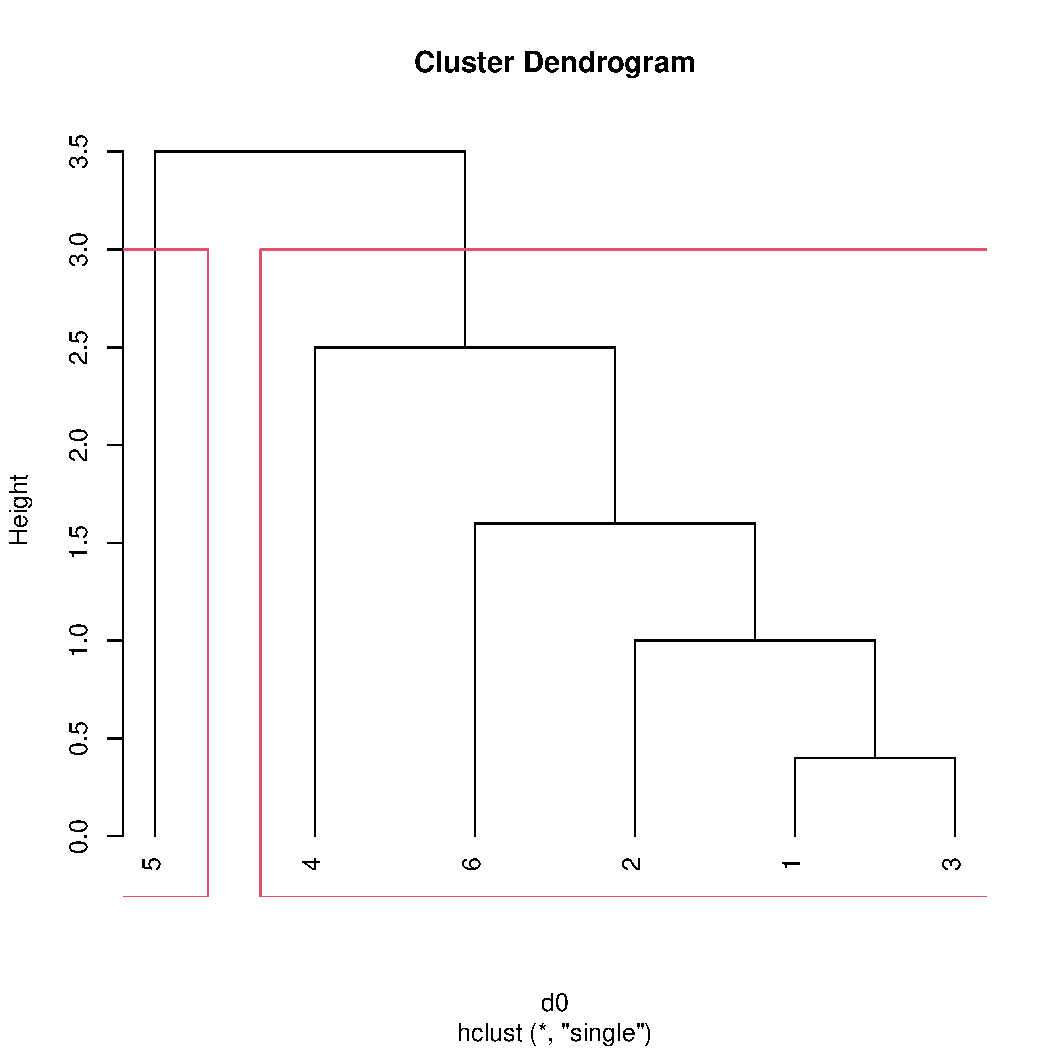
\includegraphics[scale=0.5]{7.1最短距离法.pdf}
                \caption{题1最短距离法树形图}
            \end{figure}
            \item $\pmb{x}_5^{\mathrm{T}}=(\{3,5\})$为一类,其余样品为一类。
        \end{enumerate}
        {\kaishu \textcolor{blue}{最长距离法:}}
        \begin{enumerate}[label=(\arabic*)]
            \item 聚类过程如下:\\
            六个样品自成一类$G_k=\{\pmb{x}_i^{\mathrm{T}}\}(k=1,2,\cdots,6)$,先求距离矩阵$\pmb{D}_{(0)}$。
            \begin{table}[H]
                \centering
                \begin{tabular}{|c|c|c|c|c|c|c|}
                    \hline
                    $\pmb{D}_{(0)}$ & $G_1$ & $G_2$ & $G_3$ & $G_4$ & $G_5$ & $G_6$ \\ \hline
                    $G_1$ & $0$ & & & & & \\ \hline
                    $G_2$ & $1$ & $0$ & & & & \\ \hline
                    $G_3$ & $\textit{0.4}$ & $1.4$ & $0$ & & & \\ \hline
                    $G_4$ & $2.5$ & $2.5$ & $2.5$ & $0$ & & \\ \hline
                    $G_5$ & $5.5$ & $6.5$ & $5.1$ & $6$ & $0$ & \\ \hline
                    $G_6$ & $2$ & $3$ & $1.6$ & $2.5$ & $3.5$ & $0$ \\ \hline
                \end{tabular}
            \end{table}
            $\pmb{D}_{(0)}$中最小非零元素为$0.4$,所以将对应的$G_1$和$G_3$合并为新类$G_7=G_1 \cup G_3$,按公式(7.3.4)计算新类$G_7$与其他类的距离,即$D_{7k} = \max\{D_{1k},D_{3k}\}(k= 2,4,5,6)$。其他类与类之间的距离不变,得到距离矩阵$\pmb{D}_{(1)}$。
            \begin{table}[H]
                \centering
                \begin{tabular}{|c|c|c|c|c|c|}
                    \hline
                    $\pmb{D}_{(1)}$ & $G_2$ & $G_4$ & $G_5$ & $G_6$ & $G_7$ \\ \hline
                    $G_2$ & $0$ & & & & \\ \hline
                    $G_4$ & $2.5$ & $0$ & & & \\ \hline
                    $G_5$ & $6.5$ & $6$ & $0$ & & \\ \hline
                    $G_6$ & $3$ & $2.5$ & $3.5$ & $0$ & \\ \hline
                    $G_7$ & $\textit{1.4}$ & $2.5$ & $5.5$ & $2$ & $0$ \\ \hline
                \end{tabular}
            \end{table}
            $\pmb{D}_{(1)}$中最小非零元素为$1.4$,所以将对应的$G_2$和$G_7$合并为新类$G_8=G_2 \cup G_7$,按公式(7.3.4)计算新类$G_8$与其他类的距离,即$D_{8k} = \max\{D_{2k},D_{7k}\}(k=4,5,6)$。其他类与类之间的距离不变,得到距离矩阵$\pmb{D}_{(2)}$。
            \begin{table}[H]
                \centering
                \begin{tabular}{|c|c|c|c|c|}
                    \hline
                    $\pmb{D}_{(2)}$ & $G_4$ & $G_5$ & $G_6$ & $G_8$ \\ \hline
                    $G_4$ & $0$ & & & \\ \hline
                    $G_5$ & $6$ & $0$ & & \\ \hline
                    $G_6$ & $2.5$ & $3.5$ & $0$ & \\ \hline
                    $G_8$ & $\textit{2.5}$ & $6.5$ & $3$ & $0$ \\ \hline
                \end{tabular}
            \end{table}
            $\pmb{D}_{(2)}$中最小非零元素为$2.5$,所以将对应的$G_4$和$G_8$合并为新类$G_9=G_4 \cup G_8$,计算距离矩阵$\pmb{D}_{(3)}$。
            \begin{table}[H]
                \centering
                \begin{tabular}{|c|c|c|c|c|}
                    \hline
                    $\pmb{D}_{(3)}$ & $G_5$ & $G_6$ & $G_9$ \\ \hline
                    $G_5$ & $0$ & & \\ \hline
                    $G_6$ & $3.5$ & $0$ & \\ \hline
                    $G_9$ & $6.5$ & $\textit{3}$ & $0$ \\ \hline
                \end{tabular}
            \end{table}
            $\pmb{D}_{(3)}$中最小非零元素为$3$,所以将对应的$G_6$和$G_9$合并为新类$G_{10}=G_6 \cup G_9$,计算距离矩阵$\pmb{D}_{(4)}$。
            \begin{table}[H]
                \centering
                \begin{tabular}{|c|c|c|c|c|}
                    \hline
                    $\pmb{D}_{(4)}$ & $G_5$ & $G_{10}$ \\ \hline
                    $G_5$ & $0$ & \\ \hline
                    $G_{10}$ & $\textit{6.5}$ & $0$ \\ \hline
                \end{tabular}
            \end{table}
            最后,所有样品合并为一,聚类过程结束。
            \item 树形图如下:
            \begin{figure}[H]
                \centering
                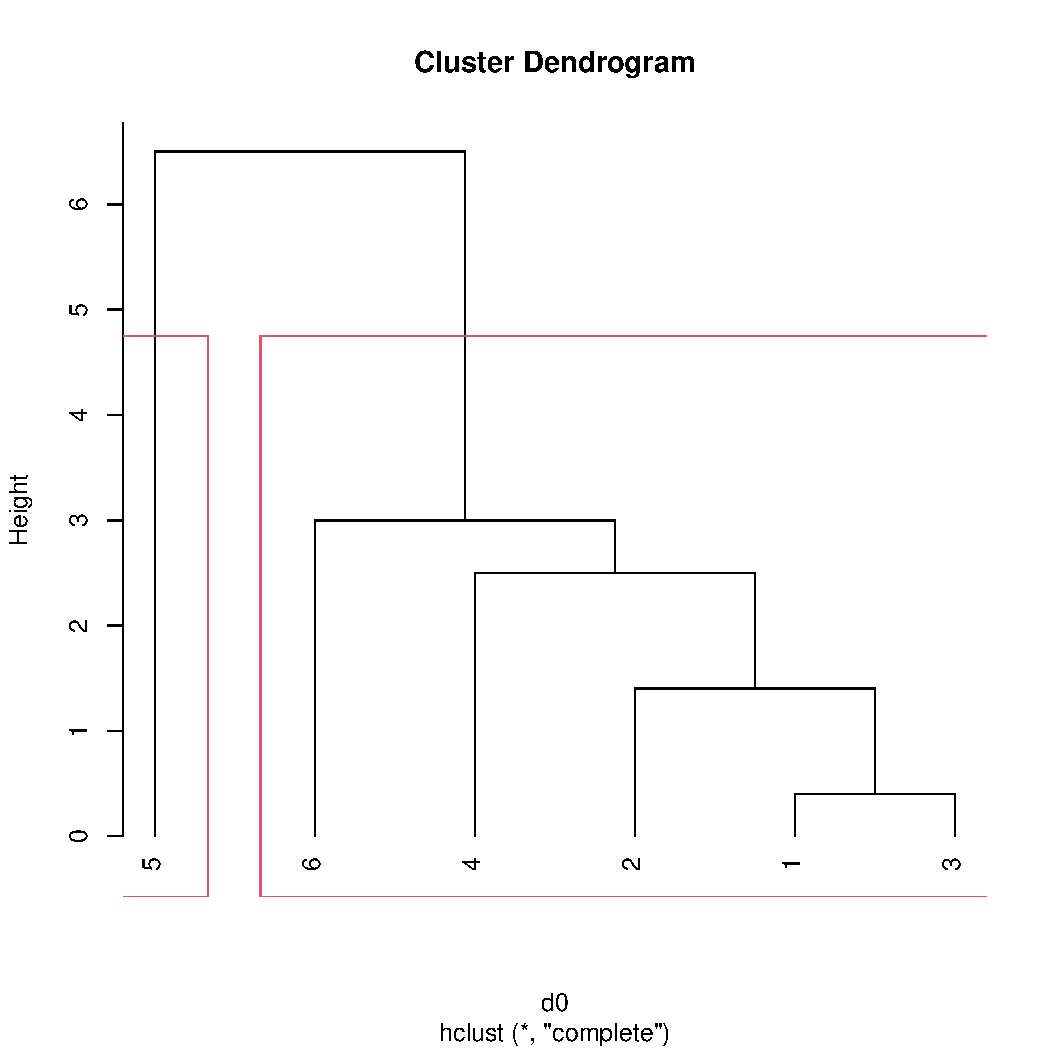
\includegraphics[scale=0.5]{7.1最长距离法.pdf}
                \caption{题1最长距离法树形图}
            \end{figure}
            \item 所以$\pmb{x}_5^{\mathrm{T}}=(\{3,5\})$为一类,其余样品为一类。
        \end{enumerate}
        \code
\begin{lstlisting}
x <- c(1,0.5,1.2,2,3,2.5,1.5,1,1.7,0,5,2.0)
dim(x) <- c(6,2)
d0 <- dist(x, method="minkowski", diag=TRUE, upper=FALSE, p=1)
# 最短距离法
hcs <- hclust(d0, method="single")
plot(hcs, hang=-1)
rect.hclust(hcs, k=2, h=NULL, border=2)
# 最长距离法
hcs <- hclust(d0, method="complete")
plot(hcs, hang=-1)
rect.hclust(hcs, k=2, h=NULL, border=2)
\end{lstlisting}
        \out\\
        输出结果见上。\\
        \summary\\
        主要结论见上。
        \item
        {\kaishu\textcolor{blue}{证:}}
        \begin{align*}
            D_{rk}^2 & =\frac{1}{n_rn_k} \sum\limits_{i \in G_r,j \in G_k}d_{ij}^2\\
            &=\frac{1}{n_rn_k}\left(\sum\limits_{i \in G_p,j \in G_k}d_{ij}^2+\sum\limits_{i \in G_q,j \in G_k}d_{ij}^2\right)\\
            &=\frac{n_p}{n_r} \cdot\frac{1}{n_pn_k} \sum\limits_{i \in G_p,j \in G_k}d_{ij}^2+\frac{n_q}{n_r} \cdot\frac{1}{n_qn_k} \sum\limits_{i \in G_q,j \in G_k}d_{ij}^2\\
            &=\frac{n_p}{n_r}D_{pk}^2+\frac{n_q}{n_r}D_{qk}^2
        \end{align*}
        \item
        {\kaishu \textcolor{blue}{解:}}\\
        {\kaishu \textcolor{blue}{最短距离法:}}
        \begin{enumerate}[label=(\arabic*)]
            \item 聚类过程如下:
            \begin{table}[H]
                \centering
                \begin{tabular}{|c|c|c|c|c|c|c|c|}
                    \hline
                    $\pmb{D}_{(0)}$ & $G_1$ & $G_2$ & $G_3$ & $G_4$ & $G_5$ & $G_6$ & $G_7$\\ \hline
                    $G_1$ & $0$ & & & & & & \\ \hline
                    $G_2$ & $4$ & $0$ & & & & & \\ \hline
                    $G_3$ & $7$ & $3$ & $0$ & & & & \\ \hline
                    $G_4$ & $12$ & $8$ & $5$ & $0$ & & & \\ \hline
                    $G_5$ & $18$ & $14$ & $11$ & $6$ & $0$ & & \\ \hline
                    $G_6$ & $19$ & $15$ & $12$ & $7$ & $\textit{1}$ & $0$ & \\ \hline
                    $G_7$ & $21$ & $17$ & $14$ & $9$ & $3$ & $2$ & $0$ \\ \hline
                \end{tabular}
            \end{table}
            \begin{table}[H]
                \centering
                \begin{tabular}{|c|c|c|c|c|c|c|}
                    \hline
                    $\pmb{D}_{(1)}$ & $G_1$ & $G_2$ & $G_3$ & $G_4$ & $G_7$ & $G_8=G_5 \cup G_6$ \\ \hline
                    $G_1$ & $0$ & & & & & \\ \hline
                    $G_2$ & $4$ & $0$ & & & & \\ \hline
                    $G_3$ & $7$ & $3$ & $0$ & & & \\ \hline
                    $G_4$ & $12$ & $8$ & $5$ & $0$ & & \\ \hline
                    $G_7$ & $21$ & $17$ & $14$ & $9$ & $0$ & \\ \hline
                    $G_8$ & $18$ & $14$ & $11$ & $6$ & $\textit{2}$ & $0$ \\ \hline
                \end{tabular}
            \end{table}
            \begin{table}[H]
                \centering
                \begin{tabular}{|c|c|c|c|c|c|}
                    \hline
                    $\pmb{D}_{(2)}$ & $G_1$ & $G_2$ & $G_3$ & $G_4$ & $G_9=G_7 \cup G_8$ \\ \hline
                    $G_1$ & $0$ & & & & \\ \hline
                    $G_2$ & $4$ & $0$ & & & \\ \hline
                    $G_3$ & $7$ & $\textit{3}$ & $0$ & & \\ \hline
                    $G_4$ & $12$ & $8$ & $5$ & $0$ & \\ \hline
                    $G_9$ & $18$ & $14$ & $11$ & $6$ & $0$ \\ \hline
                \end{tabular}
            \end{table}
            \begin{table}[H]
                \centering
                \begin{tabular}{|c|c|c|c|c|}
                    \hline
                    $\pmb{D}_{(3)}$ & $G_1$ & $G_4$ & $G_9$ & $G_{10}=G_2 \cup G_3$ \\ \hline
                    $G_1$ & $0$ & & & \\ \hline
                    $G_4$ & $12$ & $0$ & & \\ \hline
                    $G_9$ & $18$ & $6$ & $0$ & \\ \hline
                    $G_{10}$ & $\textit{4}$ & $5$ & $11$ & $0$ \\ \hline
                \end{tabular}
            \end{table}
            \begin{table}[H]
                \centering
                \begin{tabular}{|c|c|c|c|c|}
                    \hline
                    $\pmb{D}_{(4)}$ & $G_4$ & $G_9$ & $G_{11}=G_1 \cup G_{10}$ \\ \hline
                    $G_4$ & $0$ & & \\ \hline
                    $G_6$ & $6$ & $0$ & \\ \hline
                    $G_{11}$ & $\textit{5}$ & $11$ & $0$ \\ \hline
                \end{tabular}
            \end{table}
            \begin{table}[H]
                \centering
                \begin{tabular}{|c|c|c|c|c|}
                    \hline
                    $\pmb{D}_{(5)}$ & $G_9$ & $G_{12}=G_4 \cup G_{11}$ \\ \hline
                    $G_9$ & $0$ & \\ \hline
                    $G_{12}$ & $\textit{6}$ & $0$ \\ \hline
                \end{tabular}
            \end{table}
            \item 树形图如下:
            \begin{figure}[H]
                \centering
                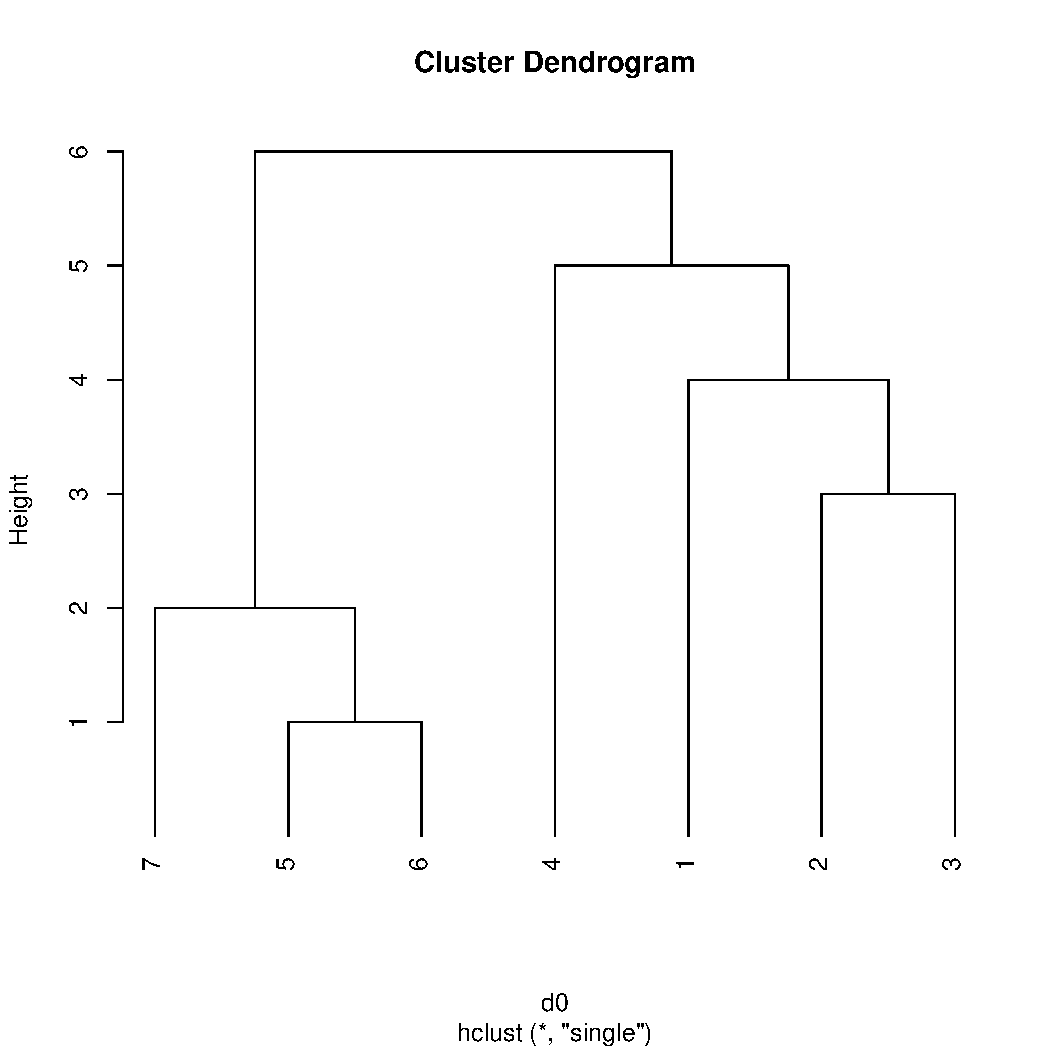
\includegraphics[scale=0.5]{7.3最短距离法.pdf}
                \caption{题3最短距离法树形图}
            \end{figure}
        \end{enumerate}
        {\kaishu \textcolor{blue}{最长距离法:}}
        \begin{enumerate}[label=(\arabic*)]
            \item 聚类过程如下:
            \begin{table}[H]
                \centering
                \begin{tabular}{|c|c|c|c|c|c|c|c|}
                    \hline
                    $\pmb{D}_{(0)}$ & $G_1$ & $G_2$ & $G_3$ & $G_4$ & $G_5$ & $G_6$ & $G_7$\\ \hline
                    $G_1$ & $0$ & & & & & & \\ \hline
                    $G_2$ & $4$ & $0$ & & & & & \\ \hline
                    $G_3$ & $7$ & $3$ & $0$ & & & & \\ \hline
                    $G_4$ & $12$ & $8$ & $5$ & $0$ & & & \\ \hline
                    $G_5$ & $18$ & $14$ & $11$ & $6$ & $0$ & & \\ \hline
                    $G_6$ & $19$ & $15$ & $12$ & $7$ & $\textit{1}$ & $0$ & \\ \hline
                    $G_7$ & $21$ & $17$ & $14$ & $9$ & $3$ & $2$ & $0$ \\ \hline
                \end{tabular}
            \end{table}
            \begin{table}[H]
                \centering
                \begin{tabular}{|c|c|c|c|c|c|c|}
                    \hline
                    $\pmb{D}_{(1)}$ & $G_1$ & $G_2$ & $G_3$ & $G_4$ & $G_7$ & $G_8=G_5 \cup G_6$ \\ \hline
                    $G_1$ & $0$ & & & & & \\ \hline
                    $G_2$ & $4$ & $0$ & & & & \\ \hline
                    $G_3$ & $7$ & $3$ & $0$ & & & \\ \hline
                    $G_4$ & $12$ & $8$ & $5$ & $0$ & & \\ \hline
                    $G_7$ & $21$ & $17$ & $14$ & $9$ & $0$ & \\ \hline
                    $G_8$ & $19$ & $15$ & $12$ & $7$ & $\textit{3}$ & $0$ \\ \hline
                \end{tabular}
            \end{table}
            \begin{table}[H]
                \centering
                \begin{tabular}{|c|c|c|c|c|c|}
                    \hline
                    $\pmb{D}_{(2)}$ & $G_1$ & $G_2$ & $G_3$ & $G_4$ & $G_9=G_7 \cup G_8$ \\ \hline
                    $G_1$ & $0$ & & & & \\ \hline
                    $G_2$ & $4$ & $0$ & & & \\ \hline
                    $G_3$ & $7$ & $\textit{3}$ & $0$ & & \\ \hline
                    $G_4$ & $12$ & $8$ & $5$ & $0$ & \\ \hline
                    $G_9$ & $21$ & $17$ & $14$ & $9$ & $0$ \\ \hline
                \end{tabular}
            \end{table}
            \begin{table}[H]
                \centering
                \begin{tabular}{|c|c|c|c|c|}
                    \hline
                    $\pmb{D}_{(3)}$ & $G_1$ & $G_4$ & $G_9$ & $G_{10}=G_2 \cup G_3$ \\ \hline
                    $G_1$ & $0$ & & & \\ \hline
                    $G_4$ & $12$ & $0$ & & \\ \hline
                    $G_9$ & $21$ & $9$ & $0$ & \\ \hline
                    $G_{10}$ & $\textit{7}$ & $8$ & $17$ & $0$ \\ \hline
                \end{tabular}
            \end{table}
            \begin{table}[H]
                \centering
                \begin{tabular}{|c|c|c|c|c|}
                    \hline
                    $\pmb{D}_{(4)}$ & $G_4$ & $G_9$ & $G_{11}=G_1 \cup G_{10}$ \\ \hline
                    $G_4$ & $0$ & & \\ \hline
                    $G_9$ & $\textit{9}$ & $0$ & \\ \hline
                    $G_{11}$ & $12$ & $21$ & $0$ \\ \hline
                \end{tabular}
            \end{table}
            \begin{table}[H]
                \centering
                \begin{tabular}{|c|c|c|c|c|}
                    \hline
                    $\pmb{D}_{(5)}$ & $G_{11}$ & $G_{12}=G_4 \cup G_9$ \\ \hline
                    $G_{11}$ & $0$ & \\ \hline
                    $G_{12}$ & $\textit{21}$ & $0$ \\ \hline
                \end{tabular}
            \end{table}
            \clearpage
            \item 树形图如下:
            \begin{figure}[H]
                \centering
                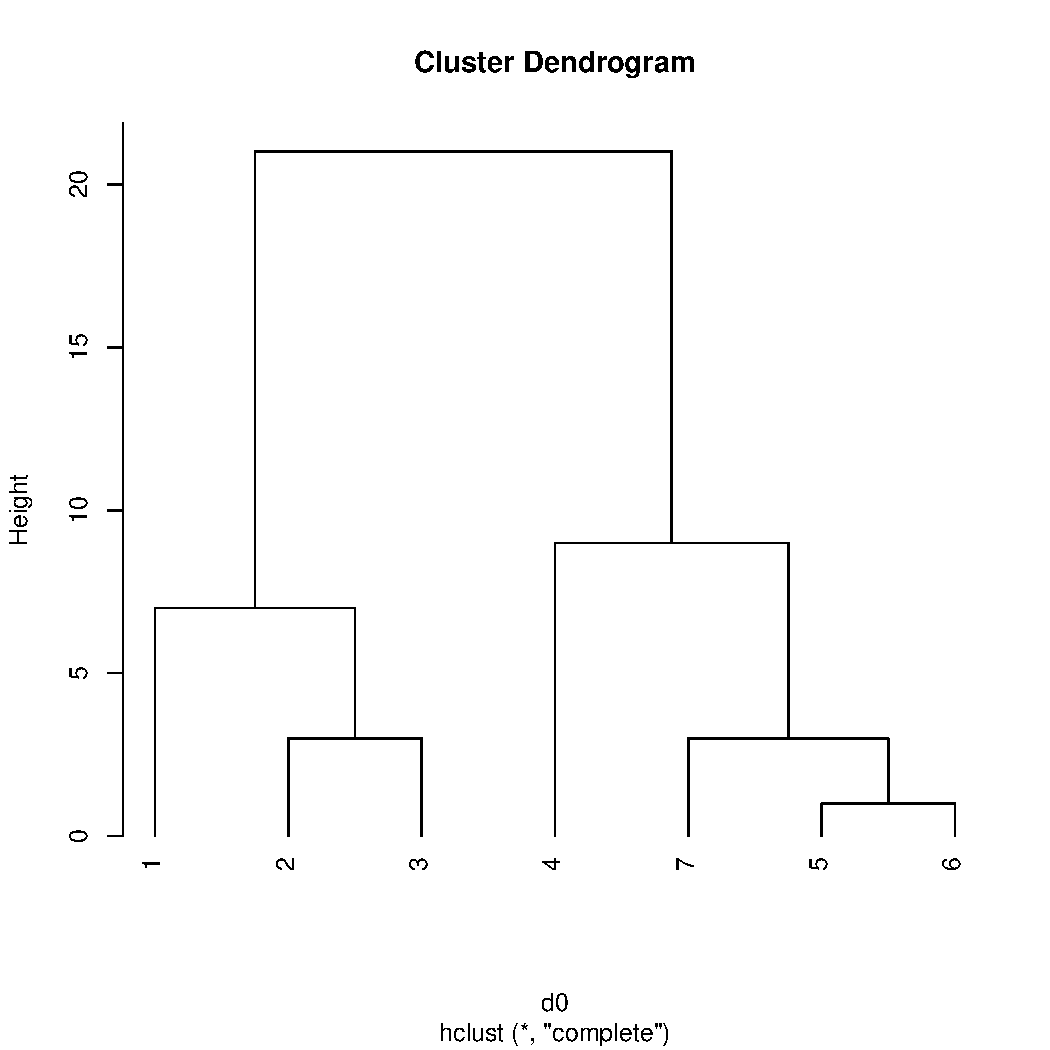
\includegraphics[scale=0.5]{7.3最长距离法.pdf}
                \caption{题3最长距离法树形图}
            \end{figure}
        \end{enumerate}
        \code
\begin{lstlisting}
D <- matrix(c(0,4,7,12,18,19,21,
              0,0,3,8,14,15,17,
              0,0,0,5,11,12,14,
              0,0,0,0,6,7,9,
              0,0,0,0,0,1,3,
              0,0,0,0,0,0,2,
              0,0,0,0,0,0,0), nr=7)
D <- D + t(D)
rownames(D) <- seq(1,7)
d0 <- as.dist(D)
# 最短距离法
hcs <- hclust(d0, method="single")
plot(hcs, hang=-1)
# 最长距离法
hcs <- hclust(d0, method="complete")
plot(hcs, hang=-1)
\end{lstlisting}
        \out\\
        输出结果如上。\\
        \summary\\
        主要结论见上。
        \item
        \code
\begin{lstlisting}
x <- read.table("ex7_4-data.txt", header=TRUE, row.names = 1)
stdx <- scale(x, center=TRUE, scale=TRUE)
# 最短距离法
d0 <- dist(x, method="euclidean", diag=TRUE, upper=FALSE)
hcs <- hclust(d0, method="single")
plot(hcs, hang=-1)
# 最长距离法
d0 <- dist(x, method="euclidean", diag=TRUE, upper=FALSE)
hcs <- hclust(d0, method="complete")
plot(hcs, hang=-1)
# 类平均法,聚为5类
d0 <- dist(x, method="euclidean", diag=TRUE, upper=FALSE)
hcs <- hclust(d0, method="average")
rect.hclust(hcs, k=5, h=NULL, border=2)
plot(hcs, hang=-1)
# 重心法,聚为5类
kmeans(stdx, 5, iter.max=10, algorithm="MacQueen")
\end{lstlisting}
        \out
        \begin{figure}[H]
            \centering
            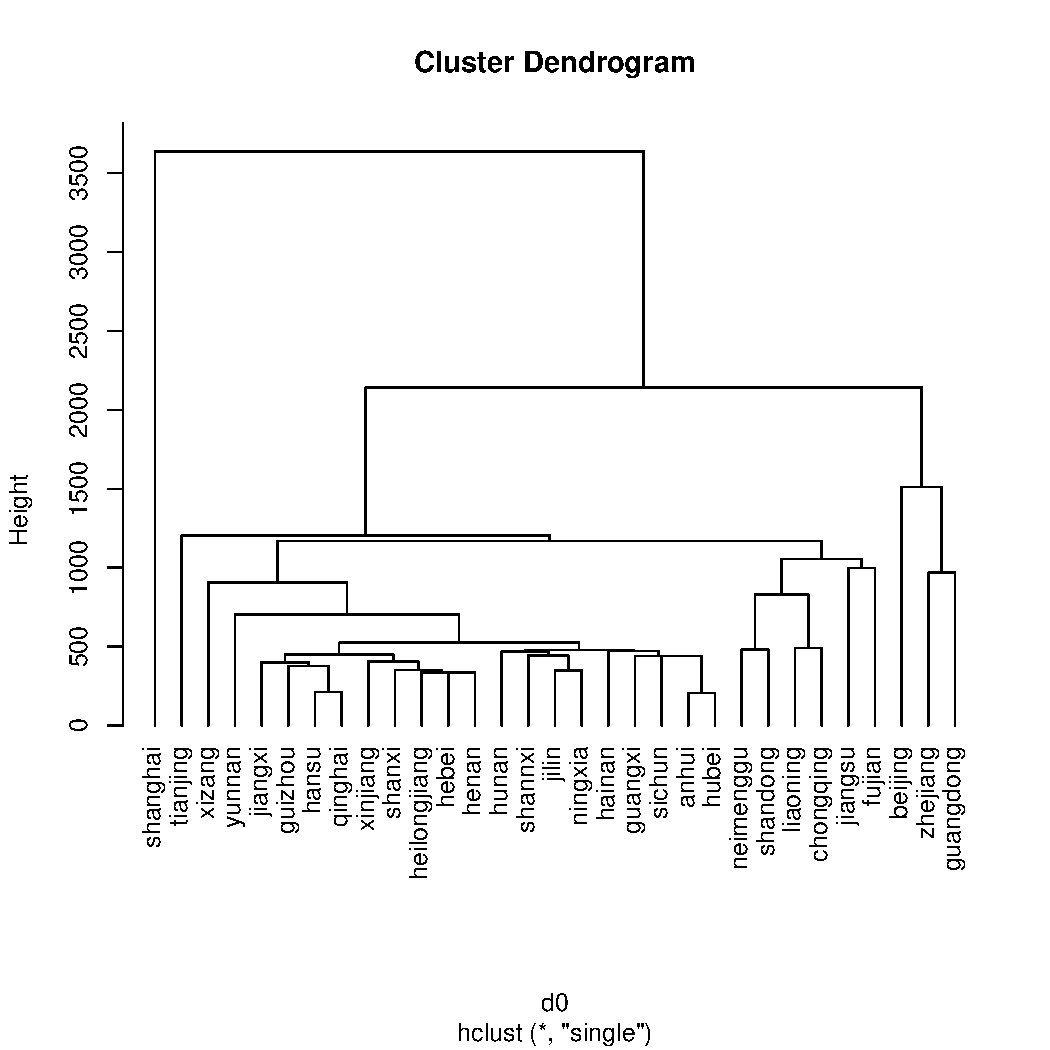
\includegraphics[scale=0.5]{7.4最短距离法.pdf}
            \caption{题4最短距离法树形图}
        \end{figure}
        \begin{figure}[H]
            \centering
            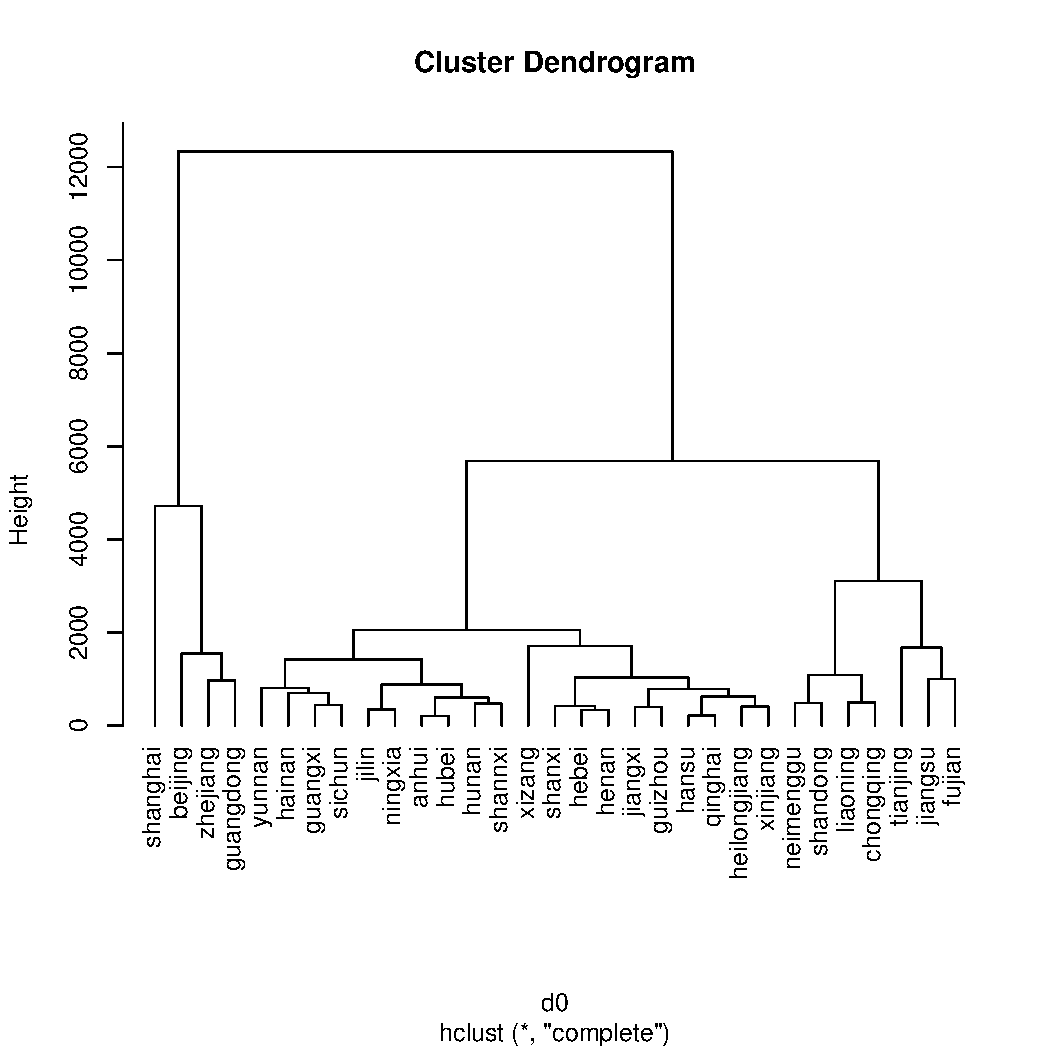
\includegraphics[scale=0.5]{7.4最长距离法.pdf}
            \caption{题4最长距离法树形图}
        \end{figure}
        \begin{figure}[H]
            \centering
            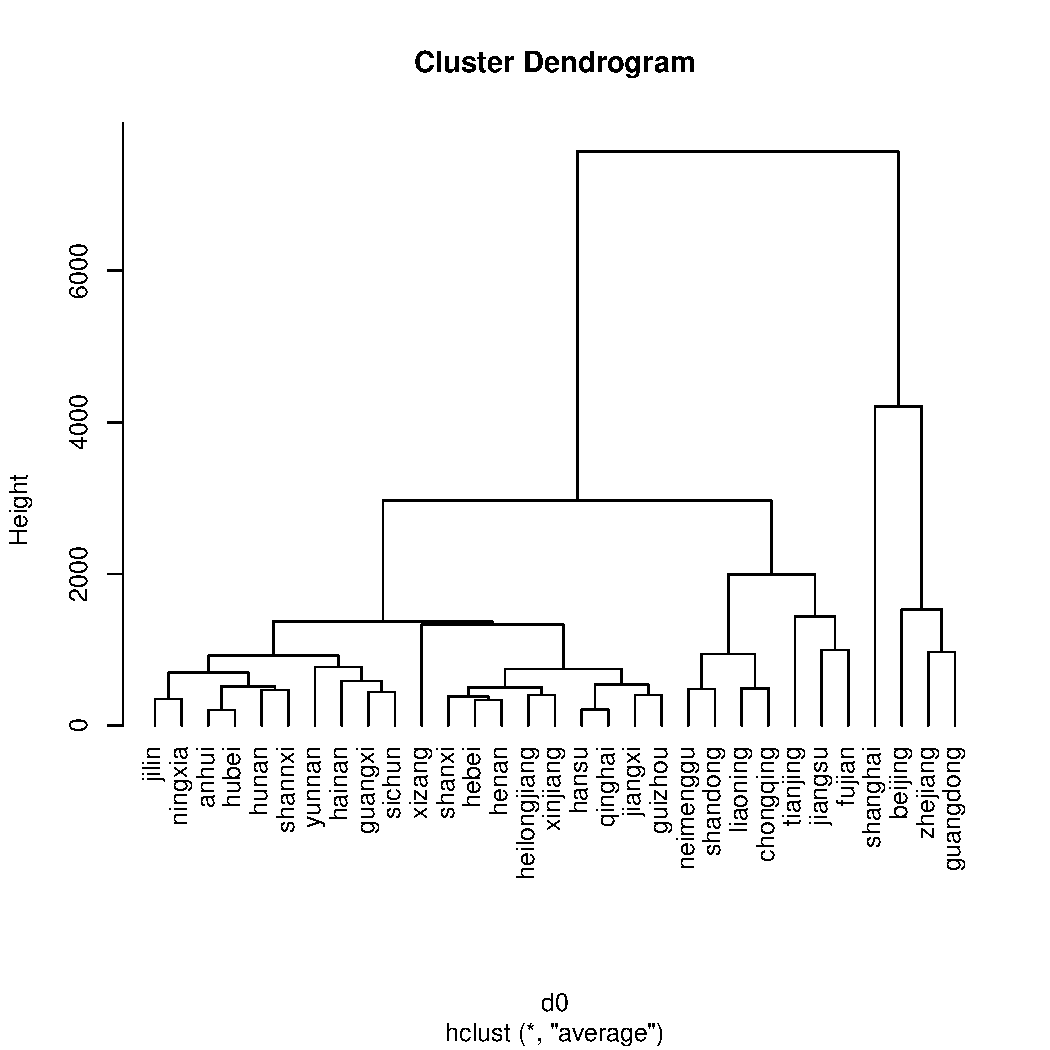
\includegraphics[scale=0.5]{7.4类平均法.pdf}
            \caption{题4类平均法树形图}
        \end{figure}
\begin{lstlisting}
> kmeans(stdx, 5, iter.max=10, algorithm="MacQueen")
K-means clustering with 5 clusters of sizes 10, 5, 3, 11, 2

Cluster means:
     xiaofei     shipin     yizhuo      juzhu jiatingshebei     yiliao   jiaotong
1 -0.4688650 -0.1858709 -0.8724430 -0.5255167   -0.29786714 -0.7981605 -0.3631822
2  1.9568033  1.7878121  0.9215928  1.6390354    1.59656427  1.3068036  1.9033693
3 -0.2694473 -0.5776927  0.2481019  0.7341867   -0.78773623  0.4678536 -0.3847263
4 -0.2592457 -0.5170184  0.3971536 -0.2012223    0.07033978  0.2332705 -0.3693902
5 -0.7176609  0.1699644 -0.4982646 -1.4645628   -1.70733938 -1.2609747 -0.3337768
      jiaoyu
1 -0.4096537
2  1.8461115
3 -0.3023638
4 -0.1503188
5 -1.2867112

Clustering vector:
     beijing     tianjing        hebei       shanxi    neimenggu     liaoning 
           2            2            4            3            4            3 
       jilin heilongjiang     shanghai      jiangsu     zhejiang        anhui 
           3            4            2            4            2            1 
      fujian      jiangxi     shandong        henan        hubei        hunan 
           1            1            4            4            1            4 
   guangdong      guangxi       hainan    chongqing       sichun      guizhou 
           2            1            1            4            1            1 
      yunnan       xizang      shannxi        hansu      qinghai      ningxia 
           5            5            4            1            1            4 
    xinjiang 
           4 

Within cluster sum of squares by cluster:
[1] 18.717017 32.974531  2.251508 19.541294  1.161091
 (between_SS / total_SS =  68.9 %)

Available components:

[1] "cluster"      "centers"      "totss"        "withinss"     "tot.withinss"
[6] "betweenss"    "size"         "iter"         "ifault"
\end{lstlisting}
        \summary\\
        主要结论如上。
        \item
        \code
\begin{lstlisting}
x <- read.table("ex7_5-data.txt", header=TRUE, row.names = 1)
stdx <- scale(x, center=TRUE, scale=TRUE)
set.seed(7)
kmeans(stdx, 5, iter.max=10, algorithm="MacQueen")
\end{lstlisting}
        \out
\begin{lstlisting}
> kmeans(stdx, 5, iter.max=10, algorithm="MacQueen")
K-means clustering with 5 clusters of sizes 11, 7, 4, 2, 7

Cluster means:
        PM10        SO2        CO2     grade2
1  0.1901517  0.2683215  0.6502499 -0.1638951
2 -0.9179291 -0.3624441  0.2052909  1.0339058
3  1.4571533  0.5235103  0.5781826 -1.7822978
4 -1.9628525 -2.1530044 -1.5680164  1.3859312
5  0.3472753  0.2567914 -1.1094977 -0.1538808

Clustering vector:
     Beijing      Tianjin Shijiazhuang      Taiyuan       Hohhot     Shenyang 
           3            1            5            5            2            5 
      Dalian       Harbin     Shanghai      Nanjing     Hangzhou        Hefei 
           2            1            1            1            1            3 
      Fuzhou     Nanchang        Jinan    Zhengzhou        Wuhan     Changsha 
           2            2            5            1            1            1 
   Guangzhou      Nanning       Haikou    Chongqing      Chengdu      Guiyang 
           2            2            4            1            1            5 
     Kunming        Lhasa        Xi'an      Lanzhou       Xining     Yinchuan 
           2            4            1            3            5            5 
      Urumqi 
           3 

Within cluster sum of squares by cluster:
[1]  6.4045158  5.6476870 16.9585359  0.3133693 10.4873904
 (between_SS / total_SS =  66.8 %)

Available components:

[1] "cluster"      "centers"      "totss"        "withinss"     "tot.withinss"
[6] "betweenss"    "size"         "iter"         "ifault"      
\end{lstlisting}
        \summary\\
        为方便固定原始随机点,使用set.seed()播撒随机数种子,根据输出可得到以下分类:
        \begin{enumerate}[label=(\arabic*)]
            \item 第1类(11个):天津、哈尔滨、上海、南京、杭州、郑州、武汉、长沙、重庆、成都、西安;
            \item 第2类(6个):呼和浩特、福州、南昌、广州、南京、昆明;
            \item 第3类(3个):北京、兰州、乌鲁木齐;
            \item 第4类(2个):海口、拉萨;
            \item 第5类(7个):石家庄、太原、沈阳、济南、贵阳、西宁、银川。
        \end{enumerate}
    \end{enumerate}
\clearpage
    \section{判别分析}
    \begin{enumerate}
        \item
        \code
\begin{lstlisting}
x1 <- read.table("ex8_1-data.txt", header=T);
x <- x1[,3:4];
G <- x1[,2];
source("distance.distinguish.R")
distance.distinguish(x, G)
\end{lstlisting}
        \out
\begin{lstlisting}
> distance.distinguish(x, G)
   G   distance blong
1  1 0.03013383     1
2  1 0.50815510     1
3  1 0.33524999     1
4  1 1.34555129     1
5  1 0.43868072     1
6  1 0.66384649     2
7  1 4.37422412     1
8  1 2.84346730     1
9  1 0.34564661     1
10 1 3.48167679     1
11 1 1.37803514     1
12 1 4.28252864     1
13 2 0.26495655     2
14 2 1.39664196     1
15 2 1.25568174     2
16 2 0.63012488     2
17 2 0.61739940     2
18 2 0.43868072     1
19 2 3.90040897     2
20 2 2.06443438     2
21 2 2.50173811     2
22 2 2.05946834     2
\end{lstlisting}
        \summary\\
        根据结果,6、14、18被误判,误判率$\displaystyle \hat{p}=\frac{3}{22} \approx 13.64\%$。
        \item
        \code
\begin{lstlisting}
library(MASS)
x <- data.matrix(iris)
colnames(x) <- c("X1", "X2", "X3", "X4", "C")
x <- data.frame(x)
discrim <- lda(C~X1+X2+X3+X4, x); discrim
p.discrim <- predict(discrim)
cbind(x[[5]], p.discrim$x, p.discrim$class)
table(x[[5]], p.discrim$class)
prop.table(table(x[[5]], p.discrim$class))
\end{lstlisting}
        \out
\begin{lstlisting}
> discrim <- lda(C~X1+X2+X3+X4, x); discrim
Call:
lda(C ~ X1 + X2 + X3 + X4, data = x)

Prior probabilities of groups:
        1         2         3 
0.3333333 0.3333333 0.3333333 

Group means:
     X1    X2    X3    X4
1 5.006 3.428 1.462 0.246
2 5.936 2.770 4.260 1.326
3 6.588 2.974 5.552 2.026

Coefficients of linear discriminants:
          LD1         LD2
X1  0.8293776  0.02410215
X2  1.5344731  2.16452123
X3 -2.2012117 -0.93192121
X4 -2.8104603  2.83918785

Proportion of trace:
   LD1    LD2 
0.9912 0.0088 
> p.discrim <- predict(discrim)
> cbind(x[[5]], p.discrim$x, p.discrim$class)
             LD1          LD2  
1   1  8.0617998  0.300420621 1
2   1  7.1286877 -0.786660426 1
3   1  7.4898280 -0.265384488 1
4   1  6.8132006 -0.670631068 1
5   1  8.1323093  0.514462530 1
6   1  7.7019467  1.461720967 1
7   1  7.2126176  0.355836209 1
8   1  7.6052935 -0.011633838 1
9   1  6.5605516 -1.015163624 1
10  1  7.3430599 -0.947319209 1
11  1  8.3973865  0.647363392 1
12  1  7.2192969 -0.109646389 1
13  1  7.3267960 -1.072989426 1
14  1  7.5724707 -0.805464137 1
15  1  9.8498430  1.585936985 1
16  1  9.1582389  2.737596471 1
17  1  8.5824314  1.834489452 1
18  1  7.7807538  0.584339407 1
19  1  8.0783588  0.968580703 1
20  1  8.0209745  1.140503656 1
21  1  7.4968023 -0.188377220 1
22  1  7.5864812  1.207970318 1
23  1  8.6810429  0.877590154 1
24  1  6.2514036  0.439696367 1
25  1  6.5589334 -0.389222752 1
26  1  6.7713832 -0.970634453 1
27  1  6.8230803  0.463011612 1
28  1  7.9246164  0.209638715 1
29  1  7.9912902  0.086378713 1
30  1  6.8294645 -0.544960851 1
31  1  6.7589549 -0.759002759 1
32  1  7.3749525  0.565844592 1
33  1  9.1263463  1.224432671 1
34  1  9.4676820  1.825226345 1
35  1  7.0620139 -0.663400423 1
36  1  7.9587624 -0.164961722 1
37  1  8.6136720  0.403253602 1
38  1  8.3304176  0.228133530 1
39  1  6.9341201 -0.705519379 1
40  1  7.6882313 -0.009223623 1
41  1  7.9179372  0.675121313 1
42  1  5.6618807 -1.934355243 1
43  1  7.2410147 -0.272615132 1
44  1  6.4144356  1.247301306 1
45  1  6.8594438  1.051653957 1
46  1  6.7647039 -0.505151855 1
47  1  8.0818994  0.763392750 1
48  1  7.1867690 -0.360986823 1
49  1  8.3144488  0.644953177 1
50  1  7.6719674 -0.134893840 1
51  2 -1.4592755  0.028543764 2
52  2 -1.7977057  0.484385502 2
53  2 -2.4169489 -0.092784031 2
54  2 -2.2624735 -1.587252508 2
55  2 -2.5486784 -0.472204898 2
56  2 -2.4299673 -0.966132066 2
57  2 -2.4484846  0.795961954 2
58  2 -0.2226665 -1.584673183 2
59  2 -1.7502012 -0.821180130 2
60  2 -1.9584224 -0.351563753 2
61  2 -1.1937603 -2.634455704 2
62  2 -1.8589257  0.319006544 2
63  2 -1.1580939 -2.643409913 2
64  2 -2.6660572 -0.642504540 2
65  2 -0.3783672  0.086638931 2
66  2 -1.2011726  0.084437359 2
67  2 -2.7681025  0.032199536 2
68  2 -0.7768540 -1.659161847 2
69  2 -3.4980543 -1.684956162 2
70  2 -1.0904279 -1.626583496 2
71  2 -3.7158961  1.044514421 3
72  2 -0.9976104 -0.490530602 2
73  2 -3.8352593 -1.405958061 2
74  2 -2.2574125 -1.426794234 2
75  2 -1.2557133 -0.546424197 2
76  2 -1.4375576 -0.134424979 2
77  2 -2.4590614 -0.935277280 2
78  2 -3.5184849  0.160588866 2
79  2 -2.5897987 -0.174611728 2
80  2  0.3074879 -1.318871459 2
81  2 -1.1066918 -1.752253714 2
82  2 -0.6055246 -1.942980378 2
83  2 -0.8987038 -0.904940034 2
84  2 -4.4984664 -0.882749915 3
85  2 -2.9339780  0.027379106 2
86  2 -2.1036082  1.191567675 2
87  2 -2.1425821  0.088779781 2
88  2 -2.4794560 -1.940739273 2
89  2 -1.3255257 -0.162869550 2
90  2 -1.9555789 -1.154348262 2
91  2 -2.4015702 -1.594583407 2
92  2 -2.2924888 -0.332860296 2
93  2 -1.2722722 -1.214584279 2
94  2 -0.2931761 -1.798715092 2
95  2 -2.0059888 -0.905418042 2
96  2 -1.1816631 -0.537570242 2
97  2 -1.6161564 -0.470103580 2
98  2 -1.4215888 -0.551244626 2
99  2  0.4759738 -0.799905482 2
100 2 -1.5494826 -0.593363582 2
101 3 -7.8394740  2.139733449 3
102 3 -5.5074800 -0.035813989 3
103 3 -6.2920085  0.467175777 3
104 3 -5.6054563 -0.340738058 3
105 3 -6.8505600  0.829825394 3
106 3 -7.4181678 -0.173117995 3
107 3 -4.6779954 -0.499095015 3
108 3 -6.3169269 -0.968980756 3
109 3 -6.3277368 -1.383289934 3
110 3 -6.8528134  2.717589632 3
111 3 -4.4407251  1.347236918 3
112 3 -5.4500957 -0.207736942 3
113 3 -5.6603371  0.832713617 3
114 3 -5.9582372 -0.094017545 3
115 3 -6.7592628  1.600232061 3
116 3 -5.8070433  2.010198817 3
117 3 -5.0660123 -0.026273384 3
118 3 -6.6088188  1.751635872 3
119 3 -9.1714749 -0.748255067 3
120 3 -4.7645357 -2.155737197 3
121 3 -6.2728391  1.649481407 3
122 3 -5.3607119  0.646120732 3
123 3 -7.5811998 -0.980722934 3
124 3 -4.3715028 -0.121297458 3
125 3 -5.7231753  1.293275530 3
126 3 -5.2791592 -0.042458238 3
127 3 -4.0808721  0.185936572 3
128 3 -4.0770364  0.523238483 3
129 3 -6.5191040  0.296976389 3
130 3 -4.5837194 -0.856815813 3
131 3 -6.2282401 -0.712719638 3
132 3 -5.2204877  1.468195094 3
133 3 -6.8001500  0.580895175 3
134 3 -3.8151597 -0.942985932 2
135 3 -5.1074897 -2.130589999 3
136 3 -6.7967163  0.863090395 3
137 3 -6.5244960  2.445035271 3
138 3 -4.9955028  0.187768525 3
139 3 -3.9398530  0.614020389 3
140 3 -5.2038309  1.144768076 3
141 3 -6.6530868  1.805319760 3
142 3 -5.1055595  1.992182010 3
143 3 -5.5074800 -0.035813989 3
144 3 -6.7960192  1.460686950 3
145 3 -6.8473594  2.428950671 3
146 3 -5.6450035  1.677717335 3
147 3 -5.1795646 -0.363475041 3
148 3 -4.9677409  0.821140550 3
149 3 -5.8861454  2.345090513 3
150 3 -4.6831543  0.332033811 3
> table(x[[5]], p.discrim$class)
   
     1  2  3
  1 50  0  0
  2  0 48  2
  3  0  1 49
> prop.table(table(x[[5]], p.discrim$class))
   
              1           2           3
  1 0.333333333 0.000000000 0.000000000
  2 0.000000000 0.320000000 0.013333333
  3 0.000000000 0.006666667 0.326666667
\end{lstlisting}
        \summary\\
        setosa全部判定正确;versicolor共50个,48个判定正确,2个误判的来自virginica;virginica共50个,49个判定正确,1个误判的来自versicolor。
        \item
        \code
\begin{lstlisting}
# 距离判别分析
x1 <- read.table("data.exam8.1.1.txt", header=T);
x <- x1[,3:6];
G <- x1[,1];
source("distance.distinguish.R")
distance.distinguish(x, G)
# 逐步判别分析
source("step.distinguish.R")
Class <- factor(x1[,1])
X <- x1[,3:6]
step.distinguish(X, Class, 3, 2)
library(MASS)
discrim <- lda(类别~蛋白质.克.+碳水化合物.克., x1)
discrim.new <- predict(discrim, x1)$class; discrim.new
\end{lstlisting}
        \out
\begin{lstlisting}
> # 距离判别分析
> distance.distinguish(x, G)
   G   distance blong
1  1  4.3787100     2
2  1  1.0525988     1
3  1  4.8132482     1
4  1  2.8991588     1
5  1  5.1404677     1
6  1  0.6086319     1
7  1  4.9104902     1
8  2  1.1025444     2
9  2  1.2821348     2
10 2  1.3082985     2
11 2  2.0305928     2
12 2  1.2567908     2
13 2  0.7929908     3
14 2  6.2835284     4
15 2  1.0467843     2
16 2  2.1486510     2
17 2  1.4494785     2
18 2  1.9106217     3
19 2  1.5017083     3
20 2  0.5803590     2
21 2  2.2790242     2
22 2  1.6158079     2
23 2  7.5244729     2
24 2  3.7590954     1
25 2 16.3220759     2
26 2  1.1933420     2
27 3  1.5832875     2
28 3  0.6001095     2
29 3  0.7715365     2
30 3  0.9989526     3
31 3  1.9371579     2
32 3  6.0741457     3
33 3  5.0845694     3
34 3  1.3260521     2
35 4  2.8151348     2
36 4  6.4970138     4
37 4  4.1744166     4
38 4  3.4092930     4
39 4  1.2765777     4
40 4  2.3049596     4
41 4  7.1090074     4
42 4  0.6855894     4
43 4  1.7329603     4

> # 逐步判别分析
> step.distinguish(X, Class, 3, 2)
$Varible
[1] "蛋白质.克."     "碳水化合物.克."

$F.Value
[1] 10.125172  9.326243

$Enter.exclude
[1] "Enter" "Enter"

$F.out.max
[1] 2.470404

$F.in.min
[1] 9.326243

$F.out
[1] 0.000000 2.470404 0.000000 1.035299
> discrim.new
 [1] 2 1 1 1 1 1 1 2 2 2 2 2 2 2 2 2 2 2 2 2 2 2 1 1 4 2 2 2 2 2 2 2 2 2 2 1 4 4 4
[40] 4 4 4 4
Levels: 1 2 3 4
\end{lstlisting}
        \summary
        \begin{enumerate}[label=(\arabic*)]
            \item 距离判别分析:1、13、14、18、19、24、31、34、35被误判。
            \item 逐步判别分析:1、23、24、25、27、28、29、30、31、32、33、34、35、36被误判。
            \item 距离判别分析法在此题的情况下误判率低于逐步判别分析法。
        \end{enumerate}
        \item
        \code
\begin{lstlisting}
ex7_4 <- function(X.origin, X.predict) {
  if (length(unique(X.origin)) != 2) {
    print("Make sure there are only two categories in the data.");
    return(NULL)
  }
  if (length(X.origin) != length(X.predict)) {
    print("Make sure the two sets of data are consistent in length.");
    return(NULL)
  }
  flag <- 0;
  for (i in seq(1, length(X.origin))) {
    if (X.origin[i] != X.predict[i]) {
      flag = flag + 1;
    }
  }
  p <- flag / length(X.origin);
  return(p)
}
\end{lstlisting}
利用题1的数据进行输出
\begin{lstlisting}
x1 <- read.table("ex8_1-data.txt", header=T);
x <- x1[,3:4];
X.origin <- x1[,2];
source("distance.distinguish.R")
X.new <- distance.distinguish(x, G)
X.new <- X.new[,3]
source("ex7_4.R")
ex7_4(X.origin, X.new)
\end{lstlisting}
        \out
\begin{lstlisting}
> ex7_4(X.origin, X.new)
[1] 0.1363636
\end{lstlisting}
        \summary\\
        在题1的数据下,误判率大致为$13.64\%$。
        \item
        \code
\begin{lstlisting}
ex7_5 <- function(data, C) {
  # data是样本数据,C是样本所属的类别,使用Fisher线性判别
  # 判断是否只有2类
  if (length(unique(C)) != 2) {
    print("Make sure there are only two categories in the data.");
    return(NULL)
  }
  # 读取数据并进行基础的命名
  m <- ncol(data);
  cols <- sprintf("X%d", seq(1:m));
  x <- cbind(C, data);
  colnames(x) <- c("C", cols);
  n <- nrow(x);
  # 进行判别
  n_wrong = 0;
  for (i in seq(1:n)) {
    x_new <- rbind(x[1:i - 1,], x[i + 1:n,]);
    discrim <- lda(C ~ ., x_new);
    p.discrim <- predict(discrim, x[i,]);
    if (p.discrim$class != x[i, 1]) {
      n_wrong = n_wrong + 1;
    }
  }
  p <- n_wrong / n;
  return(p);
}
\end{lstlisting}
利用题1的数据进行输出
\begin{lstlisting}
x1 <- read.table("ex8_1-data.txt", header=T);
data <- x1[,3:4];
C <- x1[,2];
source("ex7_5.R");
ex7_5(data, C);
\end{lstlisting}
        \out
\begin{lstlisting}
> ex7_5(data, C);
[1] 0.2272727
\end{lstlisting}
        \summary\\
        在题1的数据下,误判率大致为$22.73\% > 13.64\%$,高于回代法。在样本量偏小时,交叉确认估计误判率时准确率偏低,适用于样本量更大的情况。
    \end{enumerate}
\clearpage
    \section{相关分析}
\begin{enumerate}
    \item
    \code
\begin{lstlisting}
data <- read.table("ex9_1-data.txt", header=T, row.names = 1);
cor(data)
cor.test(~X1+X2, data=data)
cor.test(~X1+X3, data=data)
cor.test(~X1+X4, data=data)
cor.test(~X1+X5, data=data)
cor.test(~X2+X3, data=data)
cor.test(~X2+X4, data=data)
cor.test(~X2+X5, data=data)
cor.test(~X3+X4, data=data)
cor.test(~X3+X5, data=data)
cor.test(~X4+X5, data=data)
\end{lstlisting}
    \out
\begin{lstlisting}
> cor(data)
          X1          X2        X3        X4          X5
X1 1.0000000  0.33837901 0.5169851 0.8991527  0.72340083
X2 0.3383790  1.00000000 0.2772404 0.2701376 -0.05311005
X3 0.5169851  0.27724044 1.0000000 0.4255092  0.39922122
X4 0.8991527  0.27013758 0.4255092 1.0000000  0.76877136
X5 0.7234008 -0.05311005 0.3992212 0.7687714  1.00000000
> cor.test(~X1+X2, data=data)

	Pearson's product-moment correlation

data:  X1 and X2
t = 1.9365, df = 29, p-value = 0.06261
alternative hypothesis: true correlation is not equal to 0
95 percent confidence interval:
 -0.01813559  0.61855376
sample estimates:
     cor 
0.338379 

> cor.test(~X1+X3, data=data)

	Pearson's product-moment correlation

data:  X1 and X3
t = 3.2524, df = 29, p-value = 0.002901
alternative hypothesis: true correlation is not equal to 0
95 percent confidence interval:
 0.1991218 0.7364213
sample estimates:
      cor 
0.5169851 

> cor.test(~X1+X4, data=data)

	Pearson's product-moment correlation

data:  X1 and X4
t = 11.064, df = 29, p-value = 6.341e-12
alternative hypothesis: true correlation is not equal to 0
95 percent confidence interval:
 0.7995557 0.9506198
sample estimates:
      cor 
0.8991527 

> cor.test(~X1+X5, data=data)

	Pearson's product-moment correlation

data:  X1 and X5
t = 5.6423, df = 29, p-value = 4.266e-06
alternative hypothesis: true correlation is not equal to 0
95 percent confidence interval:
 0.4962694 0.8578487
sample estimates:
      cor 
0.7234008 

> cor.test(~X2+X3, data=data)

	Pearson's product-moment correlation

data:  X2 and X3
t = 1.5539, df = 29, p-value = 0.1311
alternative hypothesis: true correlation is not equal to 0
95 percent confidence interval:
 -0.08549887  0.57508563
sample estimates:
      cor 
0.2772404 

> cor.test(~X2+X4, data=data)

	Pearson's product-moment correlation

data:  X2 and X4
t = 1.5109, df = 29, p-value = 0.1416
alternative hypothesis: true correlation is not equal to 0
95 percent confidence interval:
 -0.09311562  0.56992422
sample estimates:
      cor 
0.2701376 

> cor.test(~X2+X5, data=data)

	Pearson's product-moment correlation

data:  X2 and X5
t = -0.28641, df = 29, p-value = 0.7766
alternative hypothesis: true correlation is not equal to 0
95 percent confidence interval:
 -0.3999240  0.3070076
sample estimates:
        cor 
-0.05311005 

> cor.test(~X3+X4, data=data)

	Pearson's product-moment correlation

data:  X3 and X4
t = 2.5321, df = 29, p-value = 0.01701
alternative hypothesis: true correlation is not equal to 0
95 percent confidence interval:
 0.08380479 0.67767319
sample estimates:
      cor 
0.4255092 

> cor.test(~X3+X5, data=data)

	Pearson's product-moment correlation

data:  X3 and X5
t = 2.3448, df = 29, p-value = 0.02609
alternative hypothesis: true correlation is not equal to 0
95 percent confidence interval:
 0.05227608 0.66017318
sample estimates:
      cor 
0.3992212 

> cor.test(~X4+X5, data=data)

	Pearson's product-moment correlation

data:  X4 and X5
t = 6.4735, df = 29, p-value = 4.383e-07
alternative hypothesis: true correlation is not equal to 0
95 percent confidence interval:
 0.5695918 0.8826672
sample estimates:
      cor 
0.7687714 
\end{lstlisting}
    \summary
    \begin{enumerate}[label=(\arabic*)]
        \item 各指标间的相关系数为
        \begin{table}[H]
            \centering
            \begin{tabular}{|c|c|c|c|c|c|}
                \hline
                & $X_1$ & $X_2$ & $X_3$ & $X_4$ & $X_5$ \\ \hline
                $X_1$ & 1 & 0.33837901 & 0.5169851 & 0.8991527 & 0.72340083 \\ \hline
                $X_2$ & 0.3383790 & 1 & 0.2772404 & 0.2701376 & $-0.05311005$ \\ \hline
                $X_3$ & 0.5169851 & 0.27724044 & 1 & 0.4255092 & 0.39922122 \\ \hline
                $X_4$ & 0.8991527 & 0.27013758 & 0.4255092 & 1 & 0.76877136 \\ \hline
                $X_5$ & 0.7234008 & $-0.05311005$ & 0.3992212 & 0.7687714 & 1 \\ \hline
            \end{tabular}
        \end{table}
        \item $X_1,X_2$显著性检验的$p$值为$0.06261 > 0.05$,则接受原假设,认为$X_1,X_2$不具有显著的线性相关性;
        \item $X_1,X_3$显著性检验的$p$值为$0.002901 < 0.05$,则拒绝原假设,认为$X_1,X_3$具有显著的线性相关性;
        \item $X_1,X_4$显著性检验的$p$值为$6.341\times 10^{-12} < 0.05$,则拒绝原假设,认为$X_1,X_4$具有显著的线性相关性;
        \item $X_1,X_5$显著性检验的$p$值为$4.266\times 10^{-6} < 0.05$,则拒绝原假设,认为$X_1,X_5$具有显著的线性相关性;
        \item $X_2,X_3$显著性检验的$p$值为$0.1311 > 0.05$,则接受原假设,认为$X_2,X_3$不具有显著的线性相关性;
        \item $X_2,X_4$显著性检验的$p$值为$0.1416 > 0.05$,则接受原假设,认为$X_2,X_4$不具有显著的线性相关性;
        \item $X_2,X_5$显著性检验的$p$值为$0.7766 > 0.05$,则接受原假设,认为$X_2,X_5$不具有显著的线性相关性;
        \item $X_3,X_4$显著性检验的$p$值为$0.01701 < 0.05$,则拒绝原假设,认为$X_3,X_4$具有显著的线性相关性;
        \item $X_3,X_5$显著性检验的$p$值为$0.02609 < 0.05$,则拒绝原假设,认为$X_3,X_5$具有显著的线性相关性;
        \item $X_4,X_5$显著性检验的$p$值为$4.383\times 10^{-7} < 0.05$,则拒绝原假设,认为$X_4,X_5$具有显著的线性相关性。
    \end{enumerate}
    \item
    \code
\begin{lstlisting}
# 消除X1影响,X2和X3的偏相关系数
x <- read.table("ex9_1-data.txt",head=TRUE);
x <- x[,2:6]
cor(x)
t.df <- nrow(x) - ncol(x)
ndata <- nrow(x)
nvar <- ncol(x)
r23 = (cor(x)[2, 3] - cor(x)[2, 1] * cor(x)[3, 1]) / (sqrt(1 - cor(x)[2, 1] ^ 2) * sqrt(1 - cor(x)[3, 1] ^ 2))
t <- r23 * sqrt(ndata - nvar) / sqrt(1 - r23 ^ 2)
p1 <- pt(t, t.df)
p2 <- p1 - 0.5
if (any(p2 <= 0)) p <- 2 * p1 else p <- 2 * (1 - p1)
data.frame(parial.coefs23 = r23, t = t, df = t.df, p_value = p)
# 消除X1影响,X4和X5的偏相关系数
r45 = (cor(x)[4, 5] - cor(x)[4, 1] * cor(x)[5, 1]) / (sqrt(1 - cor(x)[4, 1] ^ 2) * sqrt(1 - cor(x)[5, 1] ^ 2))
t <- r45 * sqrt(ndata - nvar) / sqrt(1 - r45 ^ 2)
p1 <- pt(t, t.df)
p2 <- p1 - 0.5
if (any(p2 <= 0)) p <- 2 * p1 else p <- 2 * (1 - p1)
data.frame(parial.coefs45 = r45, t = t, df = t.df, p_value = p)
\end{lstlisting}
    \out
\begin{lstlisting}
> data.frame(parial.coefs23 = r23, t = t, df = t.df, p_value = p)
  parial.coefs23         t df   p_value
1      0.1270064 0.6528951 26 0.5195558

> data.frame(parial.coefs45 = r45, t = t, df = t.df, p_value = p)
  parial.coefs45        t df    p_value
1      0.3915981 2.170076 26 0.03932272
\end{lstlisting}
    \summary\\
    消除$X_1$影响时,$X_2,X_3$的偏相关系数为0.1270064;\\
    消除$X_1$影响时,$X_4,X_5$的偏相关系数为0.3915981。
    \item
    \code
\begin{lstlisting}
x <- read.table("ex9_3-data.txt",head=TRUE,row.names=1);
x <- scale(x);
ca <- cancor(x[,1:2], x[,3:4]); ca
\end{lstlisting}
    \out
\begin{lstlisting}
> ca
$cor
[1] 0.7885079 0.0537397

$xcoef
        [,1]       [,2]
X1 0.1127152 -0.2789099
X2 0.1064583  0.2813576

$ycoef
        [,1]       [,2]
X3 0.1029701 -0.3610078
X4 0.1098775  0.3589657

$xcenter
           X1            X2 
 1.243450e-16 -6.049328e-16 

$ycenter
           X3            X4 
-3.380629e-16 -1.359746e-15 
\end{lstlisting}
    \summary\\
    两对典型变量为
    \[\begin{cases}
        \hat{U}_1 = 0.1127152X_1 + 0.1064583X_2,\\
        \hat{V}_1 = 0.1029701X_3 + 0.1098775X_4.
    \end{cases},\begin{cases}
        \hat{U}_2 = -0.2789099X_1 + 0.3589657X_2,\\
        \hat{V}_2 = -0.3610078X_3 + 0.3589657X_4.
    \end{cases}\]
    \item
    \code
\begin{lstlisting}
# 偏相关系数
ex9_4_partial_cor <- function(without, with, data) {
  cols <- sprintf("X%d", c(without, with));
  x <- cbind(data[,without], data[,with]);
  colnames(x) <- cols;
  rho <- cor(x);
  Mab <- det(rho[-1 * with[1], -1 * with[2]]);
  Maa <- det(rho[-1 * with[1], -1 * with[1]]);
  Mbb <- det(rho[-1 * with[2], -1 * with[2]]);
  r <- Mab / (sqrt(Maa) * sqrt(Mbb));
  return(r);
}
# 复相关系数
ex9_4_multiple_cor <- function(without, with, data) {
  cols <- sprintf("X%d", c(without, with));
  x <- cbind(data[, without], data[, with]);
  colnames(x) <- cols;
  rho <- cor(x);
  Maa <- det(rho[-1 * with[1], -1 * with[1]]);
  r <- sqrt(1 - det(rho) / Maa);
  return(r);
}
\end{lstlisting}
利用题2的前半问数据进行输出
\begin{lstlisting}
data <- read.table("ex9_1-data.txt", header=T, row.names = 1);
source("ex9_4_partial_cor.R");
ex9_4_partial_cor(c(1), c(2,3), data);
source("ex9_4_multiple_cor.R");
ex9_4_multiple_cor(c(1), c(2,3), data);
\end{lstlisting}
    \out
\begin{lstlisting}
> ex9_4_partial_cor(c(1), c(2,3), data);
[1] 0.1270064
> ex9_4_multiple_cor(c(1), c(2,3), data);
[1] 0.3588649
\end{lstlisting}
    \summary\\
    利用题2的前半问数据进行输出,故消除$X_1$影响时,$X_2,X_3$的偏相关系数为0.1270064,$X_2,X_3$的复相关系数为0.3588649。
    \item
    \code
\begin{lstlisting}
ex9_5 <- function(r, n, p, q, alpha = 0.1) {
  m <- length(r);
  Q <- rep(0, m);
  lambda <- 1
  for (k in m:1) {
    lambda <- lambda * (1 - r[k] ^ 2);
    Q[k] <- -log(lambda)
  }
  s <- 0;
  i <- m
  for (k in 1:m) {
    Q[k] <- (n - k + 1 - 1 / 2 * (p + q + 3) + s) * Q[k]
    chi <- 1 - pchisq(Q[k], (p - k + 1) * (q - k + 1))
    if (chi > alpha) {
      i <- k - 1;
      break
    }
    s <- s + 1 / r[k] ^ 2
  }
  i
}
\end{lstlisting}
    \out\\
    略。\\
    \summary\\
    略。
\end{enumerate}
\end{document}